%!TEX root = ../template.tex
%!TEX root = ../template.tex
%%%%%%%%%%%%%%%%%%%%%%%%%%%%%%%%%%%%%%%%%%%%%%%%%%%%%%%%%%%%%%%%%%%%
%% Desenvolvimento.tex
%% NOVA thesis document file
%%
%% Chapter with content
%%%%%%%%%%%%%%%%%%%%%%%%%%%%%%%%%%%%%%%%%%%%%%%%%%%%%%%%%%%%%%%%%%%%

\typeout{NT FILE Resultados.tex}%

\prependtographicspath{{Chapters/Figures/}}

% epigraph configuration
\epigraphfontsize{\small\itshape}
\setlength\epigraphwidth{12.5cm}
\setlength\epigraphrule{0pt}

\chapter{Resultados e Discussão}
\label{cha:resultados}

Neste capítulo serão discutidos os resultados obtidos com a implementação dos vários modelos. Serão apresentados, para cada modelo, o impacto que as variáveis têm nas soluções em relação à qualidade e ao tempo computacional utilizado. Também serão utilizadas instâncias de \textit{benchmark} da literatura.\\

\section{Problema de \textit{Makespan}}

Para os três modelos já apresentados existem cinco variáveis comuns com impacto na qualidade e no tempo computacional de cada solução. Desta forma, será vital encontrar uma combinação de níveis que permite obter soluções boas de forma rápida.\\
Estas cinco variáveis são: $L_{k}$, o número de iterações, ou vizinhos visitados, entre arrefecimentos; $CP$, o critério de paragem, que representa quando deve ocorrer a paragem do algoritmo; $\alpha$, a função de arrefecimento; $P$ a punição relativa à sobre-utilização de recursos; $p_{0}$, descrito como a probabilidade inicial de aceitar uma solução vizinha, algo que influência a temperatura inicial.\\
Idealmente, utilizar-se-ia $L_{k}=\infty$, $CP=\infty$, $1>\alpha\simeq1$, $p_{0}=1$. Contudo isto implicaria um tempo computacional infinito, por isso irão ser procurados outros níveis para as variáveis.\\

Os níveis apresentados na Tabela~\ref{tab:niveis_P1} foram escolhidos de forma a existir exploração da interação entre os fatores. Por outro lado, a diferença observada nos fatores $CP$ e $L_{k}$ deve-se ao facto destes serem os principais decisores do tempo computacional, a sua alteração entre modelos permitiu que o tempo computacional permanecesse comparável.\\
\begin{table}[H]
\caption{Níveis das variáveis dos modelos de \textit{Simulated Annealing}}
\label{tab:niveis_P1}
\begin{tabular}{llllll}
\hline
Modelo & $L_{k}$         & $CP$        & $\alpha$        & $P$         & $p_{0}$       \\ \hline
$M1$   & 500; 1500; 2500 & 10; 55; 100 & 0,8; 0,9; 0,975 & 10; 55; 100 & 0,5; 0,7; 0,9 \\
$M2$   & 100; 550; 1000  & 10; 55; 100 & 0,8; 0,9; 0,975 & 0           & 0,5; 0,7; 0,9 \\
$M3$   & 50; 150; 250    & 5; 30; 55   & 0,8; 0,9; 0,975 & 0           & 0,5; 0,7; 0,9 
\end{tabular}
\end{table}

Para os próximos resultados, serão considerados os exames que decorrem numa segunda-feira habitual. Ou seja, 3 cintigrafia tiroideia, 5 cintigrafia pulmonar de ventilação/inalação + perfusão, 10 cintigrafia miocárdica de perfusão em repouso, 1 cintigrafia das glândulas salivares, 10 PET - estudo corpo inteiro com FDG.\\
Os resultados obtidos são provenientes de 100 repetições de cada combinação de variáveis. Como foi possível computar paralelamente 10 repetições, os valores apresentados são a média do valor mínimo de 10 repetições. Semelhantemente, o tempo computacional aprestado é relativo à média do valor máximo de 10 repetições.\\
Todos os valores foram obtidos utilizando um processador Ryzen 5600, os modelos \textit{SA} foram executados em Python 3.11 e os modelos \textit{MILP} em Gurobi 12.0.\\

\subsection{Modelo 1}

Será agora apresentada um diagrama de calor referente ao valor da função objetivo e tempo computacional. Para a função objetivo, a faixa de cores apresentada encontra-se entre 487 e 527, sendo estes os valores da melhor solução encontrada através do \textit{MILP} e da heurística NEH, respetivamente. O tempo computacional, por sua vez teve a sua faixa de cores limitada entre 0 e 60 segundos.\\

Existem algumas observações que se podem fazer com a análise da Figura~\ref{fig:P1M1_NGV}, em relação ao impacto que cada variável tem. Observa-se a melhoria dos resultados e o aumento do tempo computacional com o aumento de $CP$ e $L_{k}$. Demonstrando novamente que estes são os principais decisores da qualidade e tempo computacional das soluções. A interação entre valores altos de temperatura inicial, devido a $p_{0}$ alto, redução lenta da temperatura, devido a $\alpha$ alto, e valores baixos de $CP$, provocam muita aceitação inicial de soluções más que não são melhoradas devido à permanência alta de temperaturas e rápida paragem do algoritmo. O aumento de $CP$ garante que se encontra uma solução igual ou melhor quando comparado a um nível de $CP$ menor, isto ocorre porque $CP$ não altera o percurso feito pelo algoritmo. O impacto do fator de punição $P$ é difícil de quantificar. Intuitivamente, quando a punição é pequena, irá ocorrer mais exploração devido ao impacto reduzido sobre a função objetivo, por outro lado, quando a punição é grande, a exploração é menor mas há mais certeza que as soluções geradas não apresentarão sobre-utilização de recursos.\\
\begin{figure}[H]
	\centering
	\begin{subfigure}{0.49\textwidth}
	\centering
		\includegraphics[width = \textwidth]{P1M1_NGV_objf}
		\caption{Média do mínimo de \textit{makespan}}
		\label{fig:P1M1_NGV_objf}
	\end{subfigure}
	\begin{subfigure}{0.49\textwidth}
	\centering
		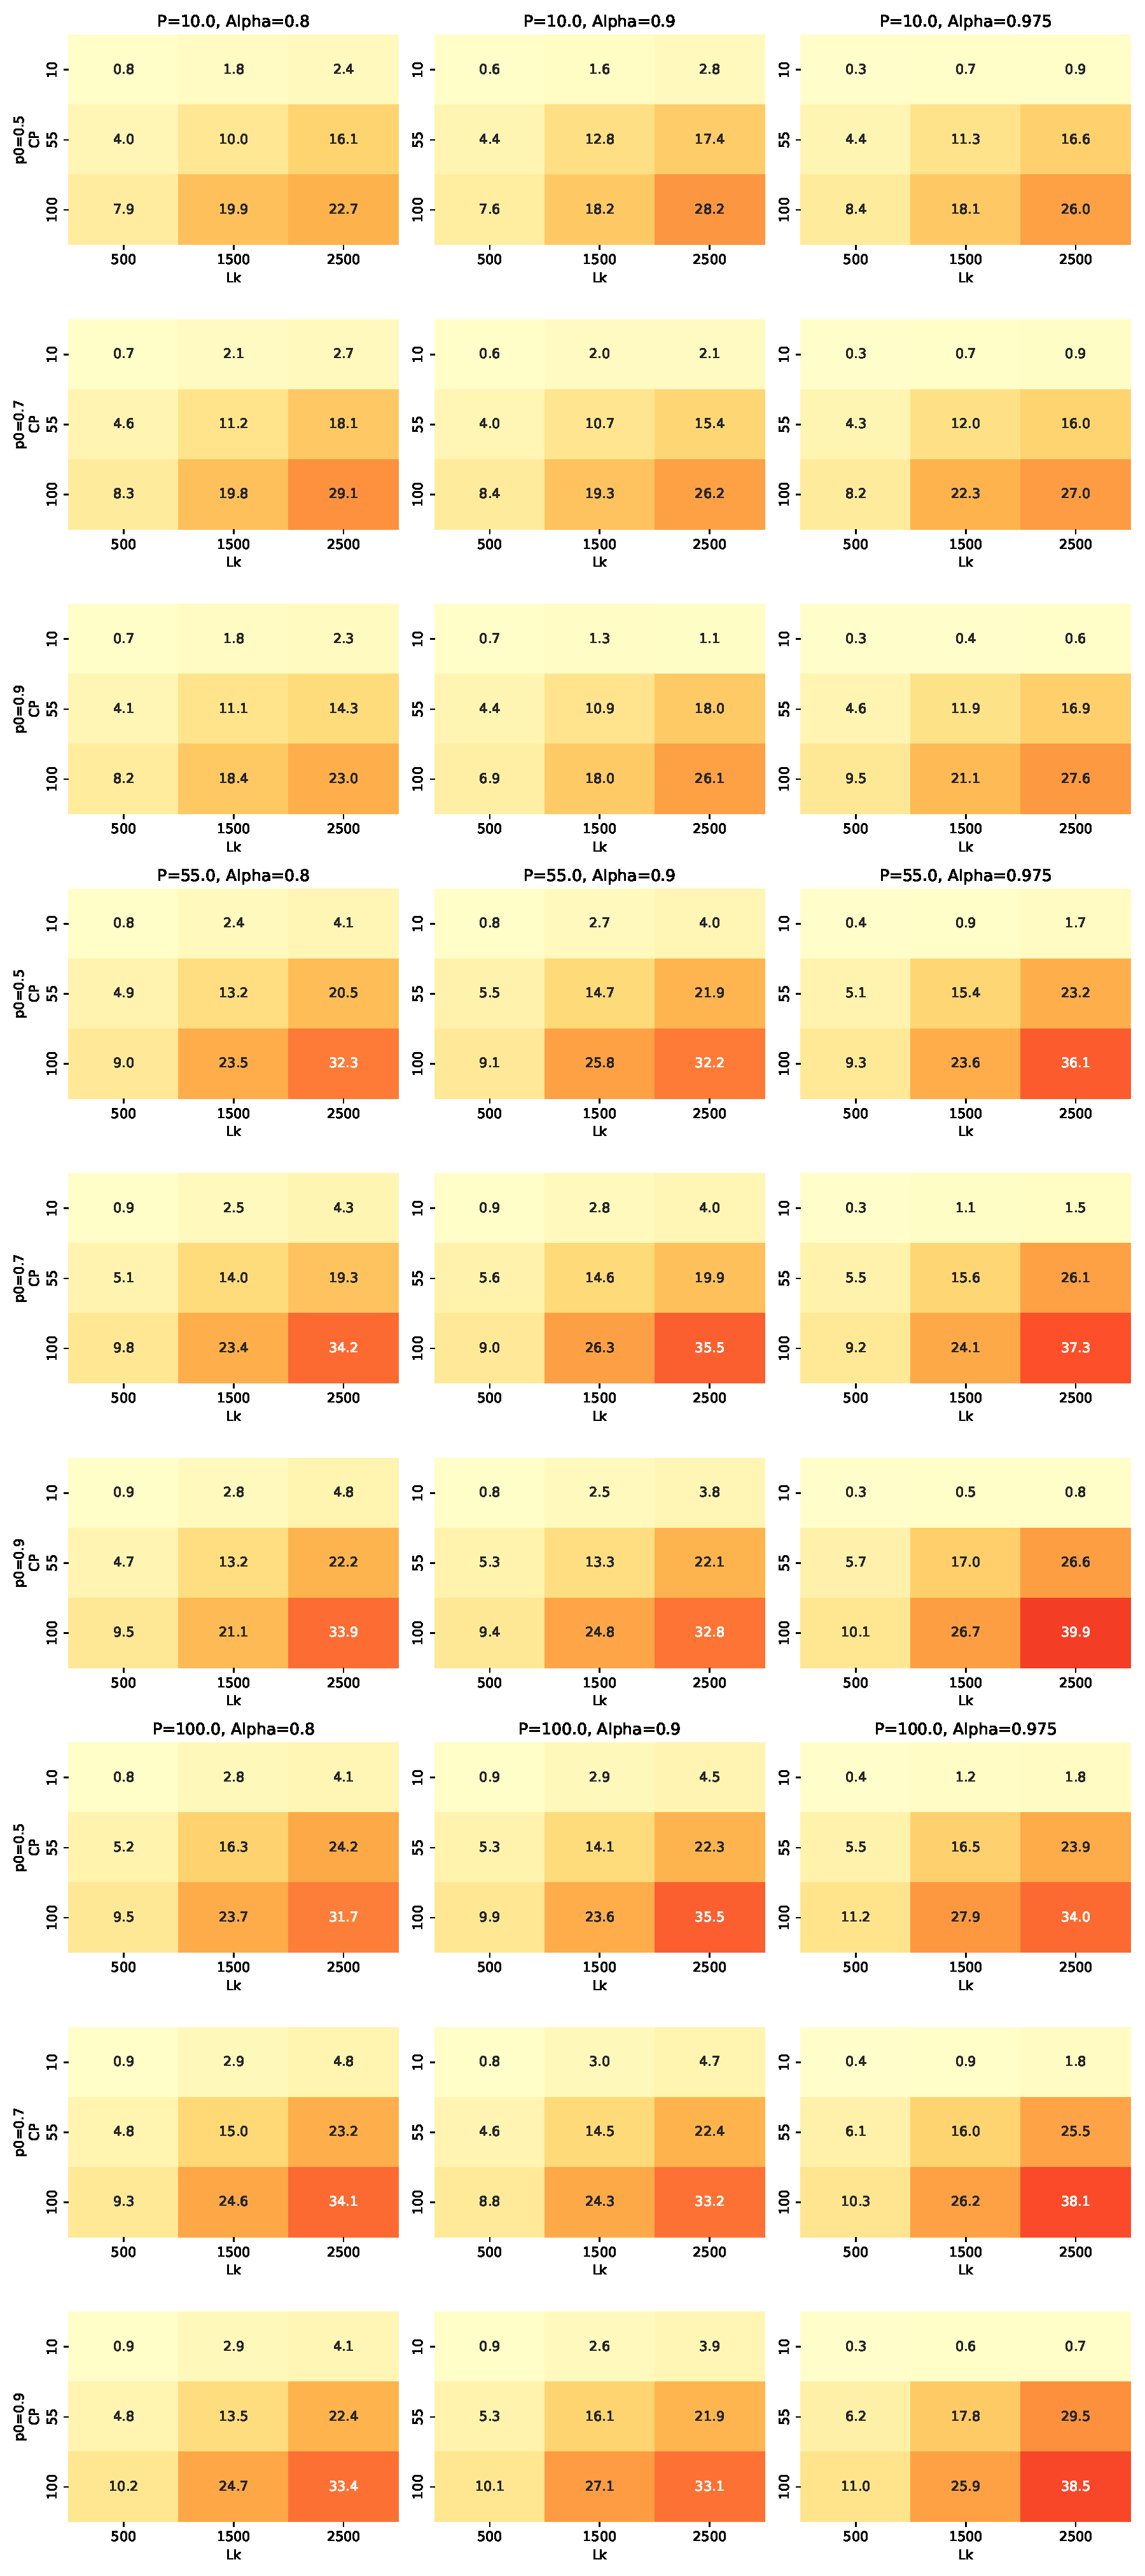
\includegraphics[width = \textwidth]{P1M1_NGV_time}
		\caption{Média do máximo do tempo de computação}
		\label{fig:P1M1_NGV_time}
	\end{subfigure}
	\caption{Impacto dos níveis das variáveis sobre o valor da função objetivo e do tempo computacional para o Modelo 1.}
	\label{fig:P1M1_NGV}
\end{figure}

Com a ajuda da Tabela~\ref{tab:P1M1_NGV_makespan} do Apêndice~\ref{chp:tabelas} pode-se tecer alguns comentários sobre os valores ótimos das variáveis primárias, em relação ao \textit{makespan}:\\
\begin{itemize}
\item $L_{k}$ não apresenta efeito linear ou quadrático significativo, o nível a escolher será aquele mais conveniente;
\item $CP$ apresenta efeito linear e quadrático significativo, ambos negativos, o nível a escolher será o alto;
\item $\alpha$ apresenta efeitos lineares e quadráticos significativos, positivo e negativo, respetivamente, o nível a escolher será o baixo;
\item $P$ apresenta efeito linear e quadrático significativo, ambos negativos, o nível a escolher será o alto;
\item $p_{0}$ apresenta efeito linear significativo positivo, o nível a escolher será o baixo.
\end{itemize}
Relativamente ao tempo, pode-se fazer uma análise semelhante pela Tabela~\ref{tab:P1M1_NGV_tempo}:
\begin{itemize}
\item $L_{k}$ apresenta efeito linear e quadrático significativos, ambos positivos, tornando difícil decidir que nível escolher, contudo intuitivamente sabe-se que reduzir $L_{k}$ deve reduzir o tempo computacional;
\item $CP$ apresenta efeito linear e quadrático significativo, ambos positivos, a escolher torna-se difícil, mas intuitivamente deve-se escolher o nível baixo;
\item $\alpha$ apresenta efeito linear positivo, o nível a escolher será o baixo;
\item $P$ apresenta efeito linear e quadrático significativo, ambos positivos, o que torna a escolha de nível difícil;
\item $p_{0}$ não apresenta efeito linear ou quadrático significativo, o nível a escolher será aquele mais conveniente.
\end{itemize}

De forma a obter uma boa combinação de variáveis, optou-se por definir uma função com ambas as variáveis dependentes a minimizar. A função é dada por:\\
$$\textit{makespan}^{10}\times \text{tempo}^{0,1}$$

Esta fórmula foi escolhida porque se pretende minimizar ambas as parcelas, \textit{makespan} e o tempo, mas também dar mais importância a pequenas diferenças entre valores de \textit{makespan}. Desta forma, a combinação que minimiza a fórmula é $\{1500; 100; 0,975; 10; 0,5\}$ com \textit{makespan} médio de 510,2 e tempo computacional médio de 18,1 segundos.\\

\subsection{Modelo 2}

Será apresentado um novo diagrama de calor referente ao \textit{makespan} e ao correspondente tempo computacional obtido através do Modelo 2 utilizando as várias combinações de níveis apresentadas na Tabela~\ref{tab:niveis_P1}. Outra vez, a faixa de cores estarão limitas aos valores já referidos. Com a análise da Figura~\ref{fig:P1M1_GV} pode-se tirar alguma conclusões acerca do impacto que cada variável tem sobre a qualidade da solução e o tempo computacional necessário.\\

Observa-se de imediato que as soluções apresentadas são melhores do que no Modelo 1, sem aumentos desproporcionais do tempo computacional, este facto é especialmente evidente por não existirem combinações de variáveis muito superiores a 527 como foi observado no Modelo 1.\\
\begin{figure}[h]
	\centering
	\begin{subfigure}{0.49\textwidth}
	\centering
		\includegraphics[width = \textwidth]{P1M1_GV_objf}
		\caption{Média do mínimo de \textit{makespan}}
		\label{fig:P1M1_GV_objf}
	\end{subfigure}
	\begin{subfigure}{0.49\textwidth}
	\centering
		\includegraphics[width = \textwidth]{P1M1_GV_time}
		\caption{Média do máximo do tempo de computação}
		\label{fig:P1M1_GV_time}
	\end{subfigure}
	\caption{Impacto dos níveis das variáveis sobre o valor da função objetivo e do tempo computacional para o Modelo 2.}
	\label{fig:P1M1_GV}
\end{figure}

Observa-se novamente o declínio da qualidade das soluções quando $CP$ é baixo, e $p_{0}$ e $\alpha$ são altos. Semelhantemente observa-se que ao aumentar $CP$ garantidamente a solução mantém-se ou melhora, o mesmo não se verifica para $L_{k}$ contudo é razoável admitir que existe a tendência para a solução melhorar.\\
Com a ajuda da Tabela~\ref{tab:P1M1_GV_makespan} pode-se comentar como se comportam as variáveis dependentes de acordo com as variáveis independentes. Relativamente ao \textit{makespan} temos que:
\begin{itemize}
\item $L_{k}$ apresenta efeito linear significativo negativo, o nível a escolher será o alto;
\item $CP$ apresenta efeito linear e quadrático significativo, ambos negativos, o nível a escolher será o alto;
\item $\alpha$ não apresenta efeito linear ou quadrático significativo, o nível a escolher será aquele mais conveniente;
\item $p_{0}$ não apresenta efeito linear ou quadrático significativo, o nível a escolher será aquele mais conveniente.
\end{itemize}
Relativamente ao tempo, pode-se fazer uma análise semelhante pela Tabela~\ref{tab:P1M1_GV_tempo}:
\begin{itemize}
\item $L_{k}$ apresenta efeito linear significativo positivo, o nível a escolher será o baixo;
\item $CP$ apresenta efeito linear e quadrático significativo, ambos positivos, a escolher torna-se difícil, mas intuitivamente devemos escolher o nível baixo;
\item $\alpha$ apresenta efeito linear significativo positivo, o nível a escolher será o baixo;
\item $p_{0}$ apresenta efeito linear significativo positivo, o nível a escolher será o baixo.
\end{itemize}

Desta forma, a combinação que minimiza a fórmula já descrita é $\{1000; 10; 0,9; 0; 0,7\}$, com \textit{makespan} médio de 506,6 e tempo computacional médio de 12,5 segundos.\\

\subsection{Modelo 3}

Será outra vez apresentado um diagrama de calor referente ao \textit{makespan} e ao tempo computacional obtido pelo Modelo 3, com os níveis descritos na Tabela~\ref{tab:niveis_P1}. A faixa de cores continua a ser limitadas como de antes. A Figura~\ref{fig:P1M2_GV} permite realizar uma análise superficial do impacto das variáveis sobre a qualidade das soluções e o tempo computacional correspondente.\\
\begin{figure}[H]
	\centering
	\begin{subfigure}{0.49\textwidth}
	\centering
		\includegraphics[width = \textwidth]{P1M2_GV_objf}
		\caption{Média do mínimo de \textit{makespan}}
		\label{fig:P1M2_GV_objf}
	\end{subfigure}
	\begin{subfigure}{0.49\textwidth}
	\centering
		\includegraphics[width = \textwidth]{P1M2_GV_time}
		\caption{Média do máximo do tempo de computação}
		\label{fig:P1M2_GV_time}
	\end{subfigure}
	\caption{Impacto dos níveis das variáveis sobre o valor da função objetivo e do tempo computacional para o Modelo 3 com \textit{left shifting}.}
	\label{fig:P1M2_GV}
\end{figure}

Na Figura~\ref{fig:P1M2_GV} observa-se de imediato que o Modelo 3 é melhor que os anteriores, apresentando soluções melhor com tempo computacional semelhante. Retiram-se as mesmo observações de antes, aumentar $CP$ garantidamente mantém ou melhora a solução, quando $CP$ é baixo, e $p_{0}$ e $\alpha$ são altos observamos soluções de pior qualidade. Pode-se analisar qual o efeito primário de cada variável sobre o \textit{makespan} utilizando a Tabela~\ref{tab:P1M2_GV_makespan}:
\begin{itemize}
\item $L_{k}$ apresenta efeito linear significativo negativo, o nível a escolher será o alto;
\item $CP$ apresenta efeito linear e quadrático significativo, ambos negativos, o nível a escolher será o alto;
\item $\alpha$ apresenta efeito linear significativo positivo, o nível a escolher será o baixo;
\item $p_{0}$ apresenta efeito linear significativo positivo, o nível a escolher será o baixo.
\end{itemize}
Para a análise sobre o tempo computacional a Tabela~\ref{tab:P1M2_GV_tempo} é utilizada: 
\begin{itemize}
\item $L_{k}$ apresenta efeito linear significativo positivo, o nível a escolher será o baixo;
\item $CP$ apresenta efeito linear e quadrático significativo, ambos positivos, a escolher torna-se difícil, mas intuitivamente devemos escolher o nível baixo;
\item $\alpha$ apresenta efeito linear e quadrático significativo, positivo e negativo, respetivamente, o nível a escolher será o baixo;
\item $p_{0}$ apresenta efeito linear significativo positivo, o nível a escolher será o baixo.
\end{itemize}

Desta forma, a combinação que minimiza a fórmula já descrita é $\{50; 5; 0,8; 0; 0,5\}$, com \textit{makespan} médio de 502,8 e tempo computacional médio de 1,5 segundos.\\

\subsection{Comparação entre modelos}

De seguida são apresentados os exames realizados em cada dia da semana no departamento de MN em estudo. Para cada um destes dias, serão utilizados os modelos já descritos para encontrar uma solução que permita minimizar o \textit{makespan}, cada modelo utilizará a combinação de níveis já definida. Além disso foram introduzidas dois algoritmos de \textit{timetabling} existentes na literatura, \textit{non-delay} (\textit{ND})~\cite{schusterApproximativeProceduresNowait2003} e \textit{enhanced non-delay} (\textit{END})~\cite{framinanEnhancedTimetablingProcedure2006}. Os Algoritmos~\ref{algo:non-delay-TT} e~\ref{algo:enh-non-delay-TT} foram utilizados para encontra os instantes no Modelo 3 \textit{ND} e \textit{END}, respetivamente. Os valores obtidos na resolução destes problemas encontram-se na Tabela~\ref{tab:P1_dias}.\\

\begin{itemize}
\item Segunda-feira: 3 cintigrafia tiroideia, 5 cintigrafia pulmonar de ventilação/inalação + perfusão, 10 cintigrafia miocárdica de perfusão em repouso, 1 cintigrafia das glândulas salivares, 10 PET - estudo corpo inteiro com FDG;
\item Terça-feira: 2 cintigrafia tiroideia, 10 cintigrafia óssea corpo inteiro, 1 cintigrafia para amiloidose cardíaca, 1 linfocintigrafia para detecção de gânglio sentinela, 2 cintigrafia pulmonar de ventilação/inalação + perfusão, 10 PET - estudo corpo inteiro com FDG;
\item Quarta-feira: 2 cintigrafia tiroideia, 2 linfocintigrafia para detecção de gânglio sentinela, 6 cintigrafia das paratiroideias, 1 tomografia cerebral com 123I-ioflupano, 3 cintigrafia pulmonar de ventilação/inalação + perfusão, 8 PET - estudo corpo inteiro com FDG;
\item Quinta-feira: 6 linfocintigrafia para detecção de gânglio sentinela, 12 cintigrafia miocárdica de perfusão em esforço/stress farmacológico, 1 tomografia cerebral com 123I-ioflupano, 2 cintigrafia miocárdica de perfusão em repouso, 10 PET - estudo corpo inteiro com FDG.
\end{itemize}


\begin{landscape}
\begin{table}[H]
\caption{Resultados provenientes dos três modelos em relação aos problemas de cada dia da semana.}
\label{tab:P1_dias}
\setlength{\tabcolsep}{2pt} % smaller horizontal padding
\begin{tabular}{llcccccccccccccccc}
\multirow{2}{*}{Dia} & \multicolumn{1}{l|}{\multirow{2}{*}{$BKS$}} & \multicolumn{3}{c|}{\textit{MILP-trad}}                                       & \multicolumn{3}{c|}{\textit{MILP-$\delta$}}                                             & \multicolumn{4}{c|}{Modelo 1}                                                                         & \multicolumn{4}{c|}{Modelo 2}                                                                         & \multicolumn{2}{c}{NEH}                     \\
                     & \multicolumn{1}{l|}{}                       & $BRPD$               & $BBRPD$              & \multicolumn{1}{c|}{$TCT$} & $BRPD$                     & $BBRPD$              & \multicolumn{1}{c|}{$TCT$} & $BRPD$               & $ARPD$                     & $TCT$                & \multicolumn{1}{c|}{$ACT$} & $BRPD$               & $ARPD$                     & $TCT$                & \multicolumn{1}{c|}{$ACT$} & $BRPD$               & $TCT$                \\ \hline
Segunda-Feira        & \multicolumn{1}{l|}{487}                    & -                    & -34,91               & \multicolumn{1}{c|}{28800} & 0,00                       & -1,64                & \multicolumn{1}{c|}{28800} & 2,87                 & 4,76                       & 104,3                & \multicolumn{1}{c|}{18,1}  & 2,26                 & 4,02                       & 94,3                 & \multicolumn{1}{c|}{12,5}  & 8,21                 & 0,17                 \\
Terça-Feira          & \multicolumn{1}{l|}{441}                    & -                    & -22,68               & \multicolumn{1}{c|}{28800} & 0,00                       & 0,00                 & \multicolumn{1}{c|}{73}    & 0,00                 & 12,15                      & 84,9                 & \multicolumn{1}{c|}{14,1}  & 0,45                 & 0,98                       & 130,8                & \multicolumn{1}{c|}{26,0}  & 4,54                 & 0,16                 \\
Quarta-Feira         & \multicolumn{1}{l|}{576}                    & -                    & -27,08               & \multicolumn{1}{c|}{28800} & 0,00                       & 0,00                 & \multicolumn{1}{c|}{19547} & 11,28                & 138,57                     & 50,0                 & \multicolumn{1}{c|}{8,1}   & 4,17                 & 4,83                       & 105,8                & \multicolumn{1}{c|}{13,4}  & 10,24                & 0,06                 \\
Quinta-Feira         & \multicolumn{1}{l|}{584}                    & -                    & -37,67               & \multicolumn{1}{c|}{28800} & 0,00                       & -4,56                & \multicolumn{1}{c|}{28800} & 3,08                 & 4,25                       & 127,3                & \multicolumn{1}{c|}{20,0}  & 2,57                 & 4,20                       & 138,3                & \multicolumn{1}{c|}{18,0}  & 10,79                & 0,32                 \\
Média                & \multicolumn{1}{l|}{}                       & -                    & -30,59               & \multicolumn{1}{c|}{28800} & 0,00                       & -1,55                & \multicolumn{1}{c|}{19305} & 4,31                 & 39,93                      & 91,6                 & \multicolumn{1}{c|}{15,1}  & 2,36                 & 3,51                       & 117,3                & \multicolumn{1}{c|}{17,5}  & 8,44                 & 0,18                 \\
                     &                                             & \multicolumn{1}{l}{} & \multicolumn{1}{l}{} & \multicolumn{1}{l}{}       & \multicolumn{1}{l}{}       & \multicolumn{1}{l}{} & \multicolumn{1}{l}{}       & \multicolumn{1}{l}{} & \multicolumn{1}{l}{}       & \multicolumn{1}{l}{} & \multicolumn{1}{l}{}       & \multicolumn{1}{l}{} & \multicolumn{1}{l}{}       & \multicolumn{1}{l}{} & \multicolumn{1}{l}{}       & \multicolumn{1}{l}{} & \multicolumn{1}{l}{} \\
                     &                                             & \multicolumn{1}{l}{} & \multicolumn{1}{l}{} & \multicolumn{1}{l}{}       & \multicolumn{1}{l}{}       & \multicolumn{1}{l}{} & \multicolumn{1}{l}{}       & \multicolumn{1}{l}{} & \multicolumn{1}{l}{}       & \multicolumn{1}{l}{} & \multicolumn{1}{l}{}       & \multicolumn{1}{l}{} & \multicolumn{1}{l}{}       & \multicolumn{1}{l}{} & \multicolumn{1}{l}{}       & \multicolumn{1}{l}{} & \multicolumn{1}{l}{} \\
\multirow{2}{*}{Dia} & \multicolumn{1}{l|}{\multirow{2}{*}{$BKS$}} & \multicolumn{4}{c|}{Modelo 3 \textit{LS}}                                            & \multicolumn{4}{c|}{Modelo 3 \textit{ELS}}                                           & \multicolumn{4}{c|}{Modelo 3 \textit{ND}}                                            & \multicolumn{4}{c}{Modelo 3 \textit{END}}                                      \\
                     & \multicolumn{1}{l|}{}                       & $BRPD$               & $ARPD$               & $TCT$                      & \multicolumn{1}{c|}{$ACT$} & $BRPD$               & $ARPD$                     & $TCT$                & \multicolumn{1}{c|}{$ACT$} & $BRPD$               & $ARPD$                     & $TCT$                & \multicolumn{1}{c|}{$ACT$} & $BRPD$               & $ARPD$                     & $TCT$                & $ACT$                \\ \hline
Segunda-Feira        & \multicolumn{1}{l|}{487}                    & 2,46                 & 3,23                 & 11,2                       & \multicolumn{1}{c|}{1,5}   & 1,64                 & 2,57                       & 20,1                 & \multicolumn{1}{c|}{3,0}   & 10,88                & 13,10                      & 5,6                  & \multicolumn{1}{c|}{0,7}   & 4,72                 & 6,51                       & 11,5                 & 1,7                  \\
Terça-Feira          & \multicolumn{1}{l|}{441}                    & 0,00                 & 0,77                 & 9,9                        & \multicolumn{1}{c|}{1,2}   & 0,00                 & 0,79                       & 13,7                 & \multicolumn{1}{c|}{1,8}   & 1,81                 & 4,10                       & 4,6                  & \multicolumn{1}{c|}{0,7}   & 1,36                 & 2,81                       & 11,7                 & 2,0                  \\
Quarta-Feira         & \multicolumn{1}{l|}{576}                    & 3,12                 & 3,59                 & 6,2                        & \multicolumn{1}{c|}{0,8}   & 0,00                 & 1,00                       & 8,9                  & \multicolumn{1}{c|}{1,4}   & 5,56                 & 7,01                       & 3,0                  & \multicolumn{1}{c|}{0,4}   & 1,74                 & 2,62                       & 7,5                  & 1,1                  \\
Quinta-Feira         & \multicolumn{1}{l|}{584}                    & 2,57                 & 3,84                 & 23,2                       & \multicolumn{1}{c|}{3,8}   & 2,23                 & 4,37                       & 33,1                 & \multicolumn{1}{c|}{5,3}   & 7,53                 & 9,49                       & 5,6                  & \multicolumn{1}{c|}{0,9}   & 4,28                 & 6,03                       & 13,9                 & 2,2                  \\ \hline
Média                & \multicolumn{1}{l|}{}                       & 2,04                 & 2,86                 & 12,6                       & \multicolumn{1}{c|}{1,8}   & 0,97                 & 2,18                       & 19,0                 & \multicolumn{1}{c|}{2,9}   & 6,45                 & 8,43                       & 4,7                  & \multicolumn{1}{c|}{0,7}   & 3,02                 & 4,49                       & 11,2                 & 1,8                 
\end{tabular}
\end{table}
\end{landscape}

Na Tabela~\ref{tab:P1_dias} observa-se a melhor solução encontrada ($BKS$), tipicamente proveniente do modelo $MILP-\delta$, o desvio relativo percentual da melhor solução ($BRPD$), o desvio relativo percentual do melhor \textit{bound} encontrado ($BBRPD$), o desvio relativo percentual médio ($ARPD$), o tempo total de computação ($TCT$), e o tempo médio de computação ($ACT$). Os valores do desvio percentual foram obtidos através da fórmula:\\
$$RPD_{h}=\frac{C_{\max}^{h}-C_{\max}^{B}}{C_{\max}^{B}}$$

Tal que $C_{\max}^{h}$ e $C_{\max}^{B}$ são os valores de \textit{makespan} obtidos pelo modelo $h$ e $BKS$. Para a obtenção das soluções, cada modelo foi executado 100 vezes, para $BRPD$ foi reportado o melhor valor encontrado e para $ARPD$ utilizou-se a média do mínimo de 10 execuções. Por sua vez, $TCT$ foi o tempo necessário para executar o modelo 100 vezes e para $ACT$ utilizou-se a média do máximo de 10 execuções.\\

Ao comparar \textit{MILP-trad} e \textit{MILP-$\delta$} observa-se a diferença entre as soluções encontradas, enquanto \textit{MILP-trad} não é capaz de chegar a uma solução admissível nas oito horas previstas, \textit{MILP-$\delta$} origina soluções ótimas ou perto de tal, tendo em conta o valor próximo de 0 de $BBRPD$.\\

Apesar da formulação \textit{MILP-$\delta$} apresentar as melhores soluções, o tempo computacional correspondente dificulta a sua utilização na prática. Também será difícil justificar a utilização do Modelo 1 ou 2, sendo que estes, em média, apresentam soluções piores com maior tempo computacional. Por sua vez, será difícil dizer que Modelo 3 com \textit{left-shifting}, \textit{enhanced left-shifting}, \textit{non-delay}, ou \textit{enhanced non-delay} apresentam soluções ou tempos estatisticamente diferentes, mas um teste estatístico com esta amostra reduzida não é viável. A heurística NEH, considerando o baixo tempo computacional utilizado, torna-se numa escolha atraente se a obtenção de uma solução razoável e rápida seja necessário.\\

Os valores referentes à melhor solução e ao tempo computacional total de cada modelo  com as várias combinações de níveis estão presentes no Apêndice~\eqref{chp:imagens}, bem como o Modelo 3 utilizando \textit{enchanced left shifting timetabling}, \textit{non-delay timetabling}, e \textit{enchanced non-delay timetabling}.

\subsection{Comparação com instâncias de \textit{benchmark}}

Nesta subsecção serão utilizados os modelos descritos anteriormente, utilizando os níveis identificados, na resolução de instâncias \textit{benchmark}. Para tal foram utilizados 21 instâncias de pequenas dimensões, com entre 6 e 10 trabalhos, e com entre 6 e 10 operações. Estas instâncias foram escolhidas devido à comparação já existente em Sundar et al.~\cite{sundarHybridArtificialBee2017}, onde também encontramos o valor da melhor solução de cada.\\

Apesar destes modelos não terem sido formulados para resolver as instâncias aqui apresentadas, sendo estes problemas apenas \textit{No-Wait Job-Shop}, é possível observar que de qualquer forma apresentam boas soluções com tempo computacional razoável. Com a análise das Tabelas~\ref{tab:P1_hipothesis_BRPD},~\ref{tab:P1_hipothesis_ARPD},~\ref{tab:P1_hipothesis_TCT},~\ref{tab:P1_hipothesis_ACT} é possível retirar algumas conclusões sobre a superioridade de alguns modelos. Realizaram-se uma série de testes de Mann–Whitney relativamente às quatro variáveis em estudo: $BRPD$, $ARPD$, $TCT$, $ACT$. Este teste pretende compara a distribuição de duas populações para a determinar se possuem a mesma distribuição. Desta forma, se o teste relativo a dois modelos for estatisticamente significante e a média de um for maior que a de outro, pode-se dizer qual destes é superior, caso contrário não podemos rejeitar que os modelos possuem a mesma distribuição.\\

Assim pode-se dizer que o Modelo 3 \textit{enhanced left-shifting} é o que apresenta as melhores soluções, dado que o teste é significante perante os restantes modelos em $BRPD$ e $ARPD$ ao mesmo tempo que apresenta a melhor média para estas variáveis. Para $TCT$ e $ACT$ o Modelo 3 \textit{enhanced left-shifting} quando comparado com os restantes modelos apresenta teste significante, em conjunto com a média indica que este apresenta tempo computacional menor sobre os Modelos 1 e 2, e maior tempo computacional sobre os restantes variantes do Modelo 3.\\

Mesmo assim, os modelos aqui descritos são inferiores aos apresentados em Sundar et al.~\cite{sundarHybridArtificialBee2017} e em Ying \& Lin~\cite{yingSolvingNowaitJobshop2020} na resolução de problemas \textit{Job-Shop with No-Wait}. O mesmo se verifica em relação ao tempo computacional, contudo esta comparação será menos relevante devido às diferentes linguagens de programação utilizadas e diferentes especificações de computadores.\\

\begin{landscape}
\begin{table}[H]
\caption{Resultados provenientes dos três modelos em relação às pequenas instâncias apresentadas em Sundar et al.~\cite{sundarHybridArtificialBee2017}.}
\label{tab:P1_instan}
\setlength{\tabcolsep}{3pt} % smaller horizontal padding
\begin{tabular}{ll|cccc|cccc|cccc|cccc}
\multirow{2}{*}{Instância} & \multirow{2}{*}{$BKS$} & \multicolumn{4}{c|}{Modelo 1}   & \multicolumn{4}{c|}{Modelo 2}   & \multicolumn{4}{c|}{Modelo 3 \textit{LS}} & \multicolumn{4}{c}{Modelo 3 \textit{ELS}} \\
                           &                        & $BRPD$ & $ARPD$ & $TCT$ & $ACT$ & $BRPD$ & $ARPD$ & $TCT$ & $ACT$ & $BRPD$  & $ARPD$ & $TCT$ & $ACT$ & $BRPD$  & $ARPD$ & $TCT$ & $ACT$ \\ \hline
Ft06                       & 73                     & 0,00   & 0,00   & 27,7  & 3,1   & 0,00   & 0,00   & 6,9   & 0,9   & 0,00    & 0,00   & 0,4   & 0,0   & 0,00    & 0,00   & 0,7   & 0,1   \\
La01                       & 971                    & 0,00   & 9,58   & 62,5  & 9,7   & 0,00   & 5,26   & 58,8  & 7,6   & 0,41    & 4,00   & 6,4   & 0,8   & 0,00    & 3,01   & 15,9  & 2,3   \\
La02                       & 937                    & 3,31   & 13,24  & 74,6  & 14,4  & 2,13   & 7,72   & 46,4  & 6,9   & 3,09    & 4,51   & 4,1   & 0,8   & 0,00    & 3,02   & 12,9  & 1,9   \\
La03                       & 820                    & 6,10   & 14,28  & 59,5  & 11,5  & 2,56   & 7,29   & 40,5  & 6,0   & 5,12    & 6,05   & 3,3   & 0,4   & 0,00    & 3,37   & 10,2  & 1,4   \\
La04                       & 887                    & 4,74   & 22,00  & 53,8  & 10,2  & 0,22   & 4,95   & 41,4  & 6,0   & 0,11    & 1,51   & 3,7   & 0,5   & 0,00    & 0,47   & 11,7  & 1,7   \\
La05                       & 777                    & 0,90   & 12,59  & 51,2  & 7,9   & 3,73   & 8,11   & 34,5  & 5,0   & 0,90    & 2,32   & 2,9   & 0,4   & 0,00    & 0,21   & 8,9   & 1,4   \\
Ft10                       & 1607                   & 12,44  & 29,56  & 150,4 & 25,3  & 1,62   & 4,84   & 256,8 & 41,9  & 0,00    & 4,92   & 21,0  & 3,0   & 0,00    & 0,45   & 61,4  & 9,9   \\
Orb01                      & 1615                   & 4,27   & 20,18  & 193,5 & 39,4  & 0,00   & 3,22   & 239,8 & 35,7  & 0,00    & 1,94   & 23,8  & 3,2   & 0,00    & 1,21   & 70,9  & 9,7   \\
Orb02                      & 1485                   & 6,13   & 30,42  & 117,6 & 26,0  & 2,22   & 4,09   & 205,2 & 29,2  & 2,22    & 2,22   & 20,2  & 3,0   & 2,22    & 2,22   & 58,9  & 8,4   \\
Orb03                      & 1599                   & 2,31   & 7,81   & 206,1 & 35,3  & 0,25   & 3,00   & 273,4 & 39,5  & 0,00    & 1,36   & 22,5  & 3,3   & 0,00    & 0,43   & 62,4  & 9,4   \\
Orb04                      & 1653                   & 12,16  & 28,68  & 135,9 & 28,0  & 4,42   & 6,64   & 289,2 & 44,6  & 4,46    & 5,89   & 26,7  & 4,3   & 0,00    & 2,27   & 71,4  & 10,5  \\
Orb05                      & 1365                   & 8,06   & 15,52  & 110,0 & 19,9  & 6,15   & 8,81   & 236,5 & 37,3  & 0,44    & 3,31   & 16,2  & 2,5   & 0,15    & 1,60   & 49,9  & 7,8   \\
Orb06                      & 1555                   & 0,00   & 10,15  & 153,4 & 24,1  & 0,00   & 2,24   & 294,7 & 42,6  & 0,00    & 0,06   & 25,2  & 3,5   & 0,00    & 0,10   & 76,6  & 11,1  \\
Orb08                      & 1319                   & 2,35   & 29,00  & 146,8 & 27,4  & 0,00   & 2,52   & 186,4 & 30,0  & 0,00    & 0,00   & 16,6  & 2,2   & 0,00    & 0,39   & 47,2  & 6,9   \\
Orb09                      & 1445                   & 6,02   & 33,88  & 119,8 & 29,5  & 0,62   & 5,97   & 225,2 & 33,6  & 4,08    & 7,31   & 20,7  & 3,0   & 0,00    & 1,68   & 59,2  & 8,4   \\
Orb10                      & 1557                   & 1,73   & 20,48  & 111,2 & 18,5  & 1,48   & 4,01   & 292,4 & 46,2  & 0,00    & 2,58   & 25,3  & 3,7   & 0,00    & 1,75   & 66,7  & 10,5  \\
La16                       & 1575                   & 4,51   & 13,74  & 134,0 & 25,2  & 0,00   & 3,59   & 283,8 & 44,2  & 1,17    & 4,72   & 22,2  & 3,1   & 0,00    & 0,78   & 69,6  & 10,3  \\
La17                       & 1371                   & 10,72  & 31,82  & 94,9  & 14,5  & 1,97   & 5,92   & 170,0 & 23,5  & 4,30    & 6,16   & 18,4  & 2,9   & 0,00    & 3,53   & 53,7  & 7,8   \\
La18                       & 1417                   & 9,81   & 25,79  & 122,4 & 27,0  & 6,35   & 9,56   & 240,8 & 35,7  & 6,35    & 6,63   & 20,6  & 3,0   & 0,00    & 5,95   & 62,0  & 9,2   \\
La19                       & 1482                   & 1,48   & 20,29  & 112,7 & 19,2  & 1,28   & 6,13   & 228,1 & 34,2  & 4,45    & 6,39   & 23,2  & 3,2   & 0,61    & 2,99   & 64,4  & 10,0  \\
La20                       & 1526                   & 10,62  & 51,03  & 132,1 & 24,1  & 5,37   & 8,29   & 284,5 & 43,5  & 0,00    & 1,80   & 24,0  & 3,5   & 0,98    & 4,92   & 72,1  & 10,3  \\ \hline
Média                      &                        & 5,13   & 20,95  & 112,9 & 21,0  & 1,92   & 5,34   & 187,4 & 28,3  & 1,77    & 3,50   & 16,5  & 2,4   & 0,19    & 1,92   & 47,9  & 7,1  
\end{tabular}
\end{table}
\end{landscape}

\begin{landscape}
\begin{table}[H]
\ContinuedFloat
\caption{Resultados provenientes dos três modelos em relação às pequenas instâncias apresentadas em Sundar et al.~\cite{sundarHybridArtificialBee2017} (continuação).}
\label{tab:P1_instan}
\setlength{\tabcolsep}{3pt} % smaller horizontal padding
\begin{tabular}{ll|cccc|cccc|cc}
\multirow{2}{*}{Instância} & \multirow{2}{*}{$BKS$} & \multicolumn{4}{c|}{Modelo 3 \text{ND}} & \multicolumn{4}{c|}{Modelo 3 \textit{END}} & \multicolumn{2}{c}{NEH} \\
                           &                        & $BRPD$  & $ARPD$ & $TCT$ & $ACT$ & $BRPD$  & $ARPD$  & $TCT$ & $ACT$ & $BRPD$      & $TCT$     \\ \hline
Ft06                       & 73                     & 0,00    & 0,00   & 0,4   & 0,1   & 0,00    & 0,00    & 0,8   & 0,1   & 0,00        & 0,0      \\
La01                       & 971                    & 7,42    & 10,24  & 4,0   & 0,4   & 6,80    & 10,05   & 8,4   & 1,0   & 31,10       & 0,0      \\
La02                       & 937                    & 7,15    & 10,28  & 1,7   & 0,2   & 0,00    & 7,03    & 5,7   & 0,8   & 21,02       & 0,0      \\
La03                       & 820                    & 5,61    & 8,59   & 1,6   & 0,2   & 4,88    & 7,83    & 4,7   & 0,7   & 23,90       & 0,0      \\
La04                       & 887                    & 0,23    & 6,60   & 1,6   & 0,2   & 1,91    & 6,46    & 4,6   & 0,6   & 5,98        & 0,0      \\
La05                       & 777                    & 5,15    & 9,94   & 1,5   & 0,2   & 5,92    & 10,10   & 3,5   & 0,5   & 10,81       & 0,0      \\
Ft10                       & 1607                   & 2,24    & 3,71   & 7,8   & 1,1   & 1,62    & 4,01    & 20,3  & 3,1   & 4,73        & 0,1      \\
Orb01                      & 1615                   & 4,64    & 5,99   & 7,4   & 1,0   & 2,72    & 4,77    & 23,6  & 3,3   & 11,95       & 0,1      \\
Orb02                      & 1485                   & 4,71    & 8,61   & 7,0   & 1,0   & 2,22    & 7,16    & 21,2  & 3,1   & 2,66        & 0,1      \\
Orb03                      & 1599                   & 1,13    & 2,46   & 6,7   & 0,9   & 0,25    & 2,51    & 21,8  & 2,9   & 17,01       & 0,1      \\
Orb04                      & 1653                   & 7,50    & 9,87   & 8,9   & 1,2   & 0,00    & 7,12    & 23,9  & 3,4   & 21,34       & 0,1      \\
Orb05                      & 1365                   & 4,18    & 8,88   & 6,0   & 0,9   & 5,71    & 7,76    & 17,0  & 2,5   & 18,02       & 0,1      \\
Orb06                      & 1555                   & 0,00    & 3,39   & 8,9   & 1,3   & 0,00    & 4,26    & 24,7  & 3,4   & 22,96       & 0,1      \\
Orb08                      & 1319                   & 0,00    & 2,47   & 6,1   & 0,8   & 0,00    & 1,08    & 17,6  & 2,4   & 7,66        & 0,0      \\
Orb09                      & 1445                   & 6,23    & 11,67  & 7,8   & 1,1   & 6,23    & 11,35   & 21,0  & 3,1   & 24,57       & 0,1      \\
Orb10                      & 1557                   & 3,92    & 9,50   & 7,8   & 1,2   & 3,92    & 8,44    & 21,5  & 3,0   & 13,04       & 0,1      \\
La16                       & 1575                   & 4,70    & 7,85   & 8,1   & 1,2   & 3,94    & 7,78    & 23,7  & 3,4   & 6,73        & 0,1      \\
La17                       & 1371                   & 5,69    & 9,87   & 6,1   & 0,9   & 1,31    & 7,78    & 16,1  & 2,2   & 17,36       & 0,1      \\
La18                       & 1417                   & 9,74    & 13,39  & 8,2   & 1,1   & 9,74    & 12,38   & 20,3  & 3,0   & 19,97       & 0,1      \\
La19                       & 1482                   & 10,32   & 13,01  & 7,7   & 1,0   & 10,12   & 13,00   & 19,9  & 2,7   & 28,41       & 0,1      \\
La20                       & 1526                   & 12,78   & 15,15  & 7,7   & 1,1   & 12,78   & 14,72   & 23,8  & 3,5   & 10,94       & 0,1      \\ \hline
Média                      &                        & 4,92    & 8,17   & 5,9   & 0,8   & 3,81    & 7,41    & 16,39 & 2,32  & 15,25       & 0,1      
\end{tabular}
\end{table}
\end{landscape}

\begin{table}[H]
\caption{Teste de Mann–Whitney de $BRPD$ para os testes realizados com as pequenas instâncias em Sundar et al.~\cite{sundarHybridArtificialBee2017}.}
\label{tab:P1_hipothesis_BRPD}
\setlength{\tabcolsep}{3pt} % smaller horizontal padding
\begin{tabular}{l|ll|ll|ll|ll|ll|ll}
                       & \multicolumn{2}{c|}{M2}            & \multicolumn{2}{c|}{M3 \textit{LS}} & \multicolumn{2}{c|}{M3 \textit{ELS}} & \multicolumn{2}{c|}{M3 \textit{ND}} & \multicolumn{2}{c|}{M3 \textit{END}} & \multicolumn{2}{c}{NEH}          \\ \hline
M1                     & \textbf{118,50} & \textbf{0,0103} & \textbf{108,50}          & \textbf{0,0047}          & \textbf{41,50}            & \textbf{0,0000}          & 218,50                   & 0,9699                   & 177,50                   & 0,2834                    & \textbf{69,50} & \textbf{0,0002} \\
M2                     & \textbf{}       & \textbf{}       & 203,00                   & 0,6630                   & \textbf{88,50}            & \textbf{0,0003}          & \textbf{111,00}          & \textbf{0,0059}          & 160,50                   & 0,1309                    & \textbf{28,00} & \textbf{0,0000} \\
M3 \textit{LS}         & \textbf{}       & \textbf{}       & \textbf{}                & \textbf{}                & \textbf{113,50}           & \textbf{0,0026}          & \textbf{100,00}          & \textbf{0,0023}          & 152,50                   & 0,0848                    & \textbf{27,00} & \textbf{0,0000} \\
M3 \textit{ELS}        & \textbf{}       & \textbf{}       & \textbf{}                & \textbf{}                & \textbf{}                 & \textbf{}                & \textbf{41,50}           & \textbf{0,0000}          & \textbf{69,00}           & \textbf{0,0000}           & \textbf{12,50} & \textbf{0,0000} \\
M3 \textit{ND}         & \textbf{}       & \textbf{}       & \textbf{}                & \textbf{}                & \textbf{}                 & \textbf{}                & \textbf{}                & \textbf{}                & 177,50                   & 0,2833                    & \textbf{63,50} & \textbf{0,0001} \\
M3 \textit{END}         & \textbf{}       & \textbf{}       & \textbf{}                & \textbf{}                & \textbf{}                 & \textbf{}                & \textbf{}                & \textbf{}                & \textbf{}                & \textbf{}                 & \textbf{52,50} & \textbf{0,0000} \\ \hline
                                 & U               & p               & U                        & p                        & U                         & p                        & U                        & p                        & U                        & p                         & U              & p              
\end{tabular}
\end{table}

\begin{table}[H]
\caption{Teste de Mann–Whitney de $ARPD$ para os testes realizados com as pequenas instâncias em Sundar et al.~\cite{sundarHybridArtificialBee2017}.}
\label{tab:P1_hipothesis_ARPD}
\setlength{\tabcolsep}{3pt} % smaller horizontal padding
\begin{tabular}{l|ll|ll|ll|ll|ll|ll}
                       & \multicolumn{2}{c|}{M2}            & \multicolumn{2}{c|}{M3 \textit{LS}} & \multicolumn{2}{c|}{M3 \textit{ELS}} & \multicolumn{2}{c|}{M3 \textit{ND}} & \multicolumn{2}{c|}{M3 \textit{END}} & \multicolumn{2}{c}{NEH}          \\ \hline
M1                               & \textbf{24,50} & \textbf{0,0000} & \textbf{20,00}           & \textbf{0,0000}          & \textbf{20,50}            & \textbf{0,0000}          & \textbf{56,50}           & \textbf{0,0000}          & \textbf{43,50}           & \textbf{0,0000}           & 153,50          & 0,0943          \\
M2                               & \textbf{}      & \textbf{}       & \textbf{130,00}          & \textbf{0,0236}          & \textbf{56,50}            & \textbf{0,0000}          & \textbf{114,50}          & \textbf{0,0080}          & 143,00                   & 0,0527                    & \textbf{70,50}  & \textbf{0,0002} \\
M3 \textit{LS}  & \textbf{}      & \textbf{}       & \textbf{}                & \textbf{}                & \textbf{138,00}           & \textbf{0,0391}          & \textbf{71,00}           & \textbf{0,0002}          & \textbf{80,00}           & \textbf{0,0004}           & \textbf{44,00}  & \textbf{0,0000} \\
M3 \textit{ELS} & \textbf{}      & \textbf{}       & \textbf{}                & \textbf{}                & \textbf{}                 & \textbf{}                & \textbf{39,50}           & \textbf{0,0000}          & \textbf{46,50}           & \textbf{0,0000}           & \textbf{29,50}  & \textbf{0,0000} \\
M3 \textit{ND}  & \textbf{}      & \textbf{}       & \textbf{}                & \textbf{}                & \textbf{}                 & \textbf{}                & \textbf{}                & \textbf{}                & 185,50                   & 0,3854                    & \textbf{111,50} & \textbf{0,0063} \\
M3 \textit{END} & \textbf{}      & \textbf{}       & \textbf{}                & \textbf{}                & \textbf{}                 & \textbf{}                & \textbf{}                & \textbf{}                & \textbf{}                & \textbf{}                 & \textbf{106,50} & \textbf{0,0043} \\ \hline
                                 & U              & p               & U                        & p                        & U                         & p                        & U                        & p                        & U                        & p                         & U               & p              
\end{tabular}
\end{table}

\begin{table}[H]
\caption{Teste de Mann–Whitney de $TCT$ para os testes realizados com as pequenas instâncias em Sundar et al.~\cite{sundarHybridArtificialBee2017}.}
\label{tab:P1_hipothesis_TCT}
\setlength{\tabcolsep}{3pt} % smaller horizontal padding
\begin{tabular}{l|ll|ll|ll|ll|ll|ll}
                       & \multicolumn{2}{c|}{M2}            & \multicolumn{2}{c|}{M3 \textit{LS}} & \multicolumn{2}{c|}{M3 \textit{ELS}} & \multicolumn{2}{c|}{M3 \textit{ND}} & \multicolumn{2}{c|}{M3 \textit{END}} & \multicolumn{2}{c}{NEH}          \\ \hline
M1                               & \textbf{124,00} & \textbf{0,0157} & \textbf{0,00}            & \textbf{0,0000}          & \textbf{58,00}           & \textbf{0,0000}           & \textbf{0,00}            & \textbf{0,0000}          & \textbf{0,00}            & \textbf{0,0000}           & \textbf{0,00} & \textbf{0,0000} \\
M2                               & \textbf{}       & \textbf{}       & \textbf{15,00}           & \textbf{0,0000}          & \textbf{92,00}           & \textbf{0,0013}           & \textbf{11,00}           & \textbf{0,0000}          & \textbf{16,00}           & \textbf{0,0000}           & \textbf{0,00} & \textbf{0,0000} \\
M3 \textit{LS}  & \textbf{}       & \textbf{}       & \textbf{}                & \textbf{}                & \textbf{95,00}           & \textbf{0,0017}           & \textbf{95,50}           & \textbf{0,0017}          & 211,00                   & 0,8209                    & \textbf{1,00} & \textbf{0,0000} \\
M3 \textit{ELS} & \textbf{}       & \textbf{}       & \textbf{}                & \textbf{}                & \textbf{}                & \textbf{}                 & \textbf{21,00}           & \textbf{0,0000}          & \textbf{96,00}           & \textbf{0,0018}           & \textbf{1,00} & \textbf{0,0000} \\
M3 \textit{ND}  & \textbf{}       & \textbf{}       & \textbf{}                & \textbf{}                & \textbf{}                & \textbf{}                 & \textbf{}                & \textbf{}                & \textbf{83,00}           & \textbf{0,0006}           & \textbf{1,00} & \textbf{0,0000} \\
M3 \textit{END} & \textbf{}       & \textbf{}       & \textbf{}                & \textbf{}                & \textbf{}                & \textbf{}                 & \textbf{}                & \textbf{}                & \textbf{}                & \textbf{}                 & \textbf{1,00} & \textbf{0,0000} \\ \hline
                                 & U               & p               & U                        & p                        & U                        & p                         & U                        & p                        & U                        & p                         & U             & p              
\end{tabular}
\end{table}

\begin{table}[H]
\caption{Teste de Mann–Whitney de $ACT$ para os testes realizados com as pequenas instâncias em Sundar et al.~\cite{sundarHybridArtificialBee2017}.}
\label{tab:P1_hipothesis_ACT}
\setlength{\tabcolsep}{3pt} % smaller horizontal padding
\begin{tabular}{l|ll|ll|ll|ll|ll|ll}
                       & \multicolumn{2}{c|}{M2}            & \multicolumn{2}{c|}{M3 \textit{LS}} & \multicolumn{2}{c|}{M3 \textit{ELS}} & \multicolumn{2}{c|}{M3 \textit{ND}} & \multicolumn{2}{c|}{M3 \textit{END}} & \multicolumn{2}{c}{NEH}          \\ \hline
M1                               & 144,00     & 0,0559    & \textbf{7,50}            & \textbf{0,0000}          & \textbf{39,50}           & \textbf{0,0000}           & \textbf{0,00}            & \textbf{0,0000}          & \textbf{6,50}            & \textbf{0,0000}           & \textbf{0,00}  & \textbf{0,0000} \\
M2                               & \textbf{}  & \textbf{} & \textbf{15,00}           & \textbf{0,0000}          & \textbf{93,50}           & \textbf{0,0015}           & \textbf{12,50}           & \textbf{0,0000}          & \textbf{16,00}           & \textbf{0,0000}           & \textbf{1,00}  & \textbf{0,0000} \\
M3 \textit{LS}  & \textbf{}  & \textbf{} & \textbf{}                & \textbf{}                & \textbf{94,00}           & \textbf{0,0015}           & \textbf{96,00}           & \textbf{0,0018}          & 209,00                   & 0,7814                    & \textbf{25,50} & \textbf{0,0000} \\
M3 \textit{ELS} & \textbf{}  & \textbf{} & \textbf{}                & \textbf{}                & \textbf{}                & \textbf{}                 & \textbf{20,50}           & \textbf{0,0000}          & \textbf{94,50}           & \textbf{0,0016}           & \textbf{2,00}  & \textbf{0,0000} \\
M3 \textit{ND}  & \textbf{}  & \textbf{} & \textbf{}                & \textbf{}                & \textbf{}                & \textbf{}                 & \textbf{}                & \textbf{}                & \textbf{89,50}           & \textbf{0,0010}           & \textbf{11,00} & \textbf{0,0000} \\
M3 \textit{END} & \textbf{}  & \textbf{} & \textbf{}                & \textbf{}                & \textbf{}                & \textbf{}                 & \textbf{}                & \textbf{}                & \textbf{}                & \textbf{}                 & \textbf{6,00}  & \textbf{0,0000} \\ \hline
                                 & U          & p         & U                        & p                        & U                        & p                         & U                        & p                        & U                        & p                         & U              & p              
\end{tabular}
\end{table}



\section{Problema do número de trabalhos}

Para os três modelos já apresentados deste problema, existem cinco variáveis a estudar relativamente ao seu impacto sobre a qualidade da solução e o tempo computacional necessário. Os níveis de cada variável estudados para os modelos são reportados na Tabela~\ref{tab:niveis_P2}. Os níveis de $L_{k}$ e $CP$ utilizados foram concebidos de forma a manter o tempo computacional semelhante entre os modelos. Por sua vez, os níveis da punição $P$ são menores que os utilizados no problema de \textit{makespan}, devido ao menor ótimo da função objetivo.\\
\begin{table}[H]
\caption{Níveis das variáveis dos modelos de \textit{Simulated Annealing}}
\label{tab:niveis_P2}
\begin{tabular}{llllll}
\hline
Modelo & $L_{k}$          & $CP$        & $\alpha$        & $P$      & $p_{0}$       \\ \hline
$M1$   & 1000; 3000; 5000 & 30; 90; 150 & 0,8; 0,9; 0,975 & 1; 5; 10 & 0,5; 0,7; 0,9 \\
$M2$   & 100; 500; 1000   & 10; 55; 100 & 0,8; 0,9; 0,975 & 0        & 0,5; 0,7; 0,9 \\
$M3$   & 50; 150; 250     & 5; 30; 55   & 0,8; 0,9; 0,975 & 0        & 0,5; 0,7; 0,9
\end{tabular}
\end{table}

Para os próximos resultados, serão considerados o dobro dos exames que decorrem numa segunda-feira habitual. Ou seja, 6 cintigrafia tiroideia, 10 cintigrafia pulmonar de ventilação/inalação + perfusão, 20 cintigrafia miocárdica de perfusão em repouso, 2 cintigrafia das glândulas salivares, 20 PET - estudo corpo inteiro com FDG. Para o valor de $T_{\max}$ será utilizado o melhor valor de \textit{makespan} encontrado no problema anterior, ou seja, de 487 minutos.\\
Os resultados obtidos são provenientes de 100 repetições de cada combinação de variáveis. Como foi possível computar paralelamente 10 repetições, os valores apresentados são a média do valor mínimo de 10 repetições. Semelhantemente, o tempo computacional aprestado é relativo à média do valor máximo de 10 repetições.\\

\subsection{Modelo 1}

Será apresentado um diagrama de calor referente ao valor da função objetivo e tempo computacional. Para a função objetivo, a faixa de cores está limitada aos valores entre -34 e -29, sendo estes os valores da melhor solução encontrada pelo \textit{MILP-$\delta$} e pela heurística NEH, respetivamente. O tempo computacional também está limitada entre 0 e 60 segundos.\\

Com a Figura~\ref{fig:P2M1_NNGV} pode-se tecer alguns comentários. A combinação de $CP$ baixo e redução lenta de temperatura diminui a qualidade das soluções. O aumento do nível de $CP$ garante que a solução se mantém ou melhora. Por sua vez, o aumento de $L_{k}$ tende a melhorar a solução, contudo não existe a garantia de tal. A punição $P$ não aparenta ter grande impacto sobre a qualidade da solução quando $\alpha$ e $p_{0}$ são baixos, mas quando estes níveis são elevados, o aumento de $P$ parece piorar as soluções. Relativamente ao tempo computacional, os principais decisores aparentam ser $L_{k}$ e $Cp$, quando estes níveis aumentam também aumenta o tempo computacional.\\
\begin{figure}[H]
	\centering
	\begin{subfigure}{0.49\textwidth}
	\centering
		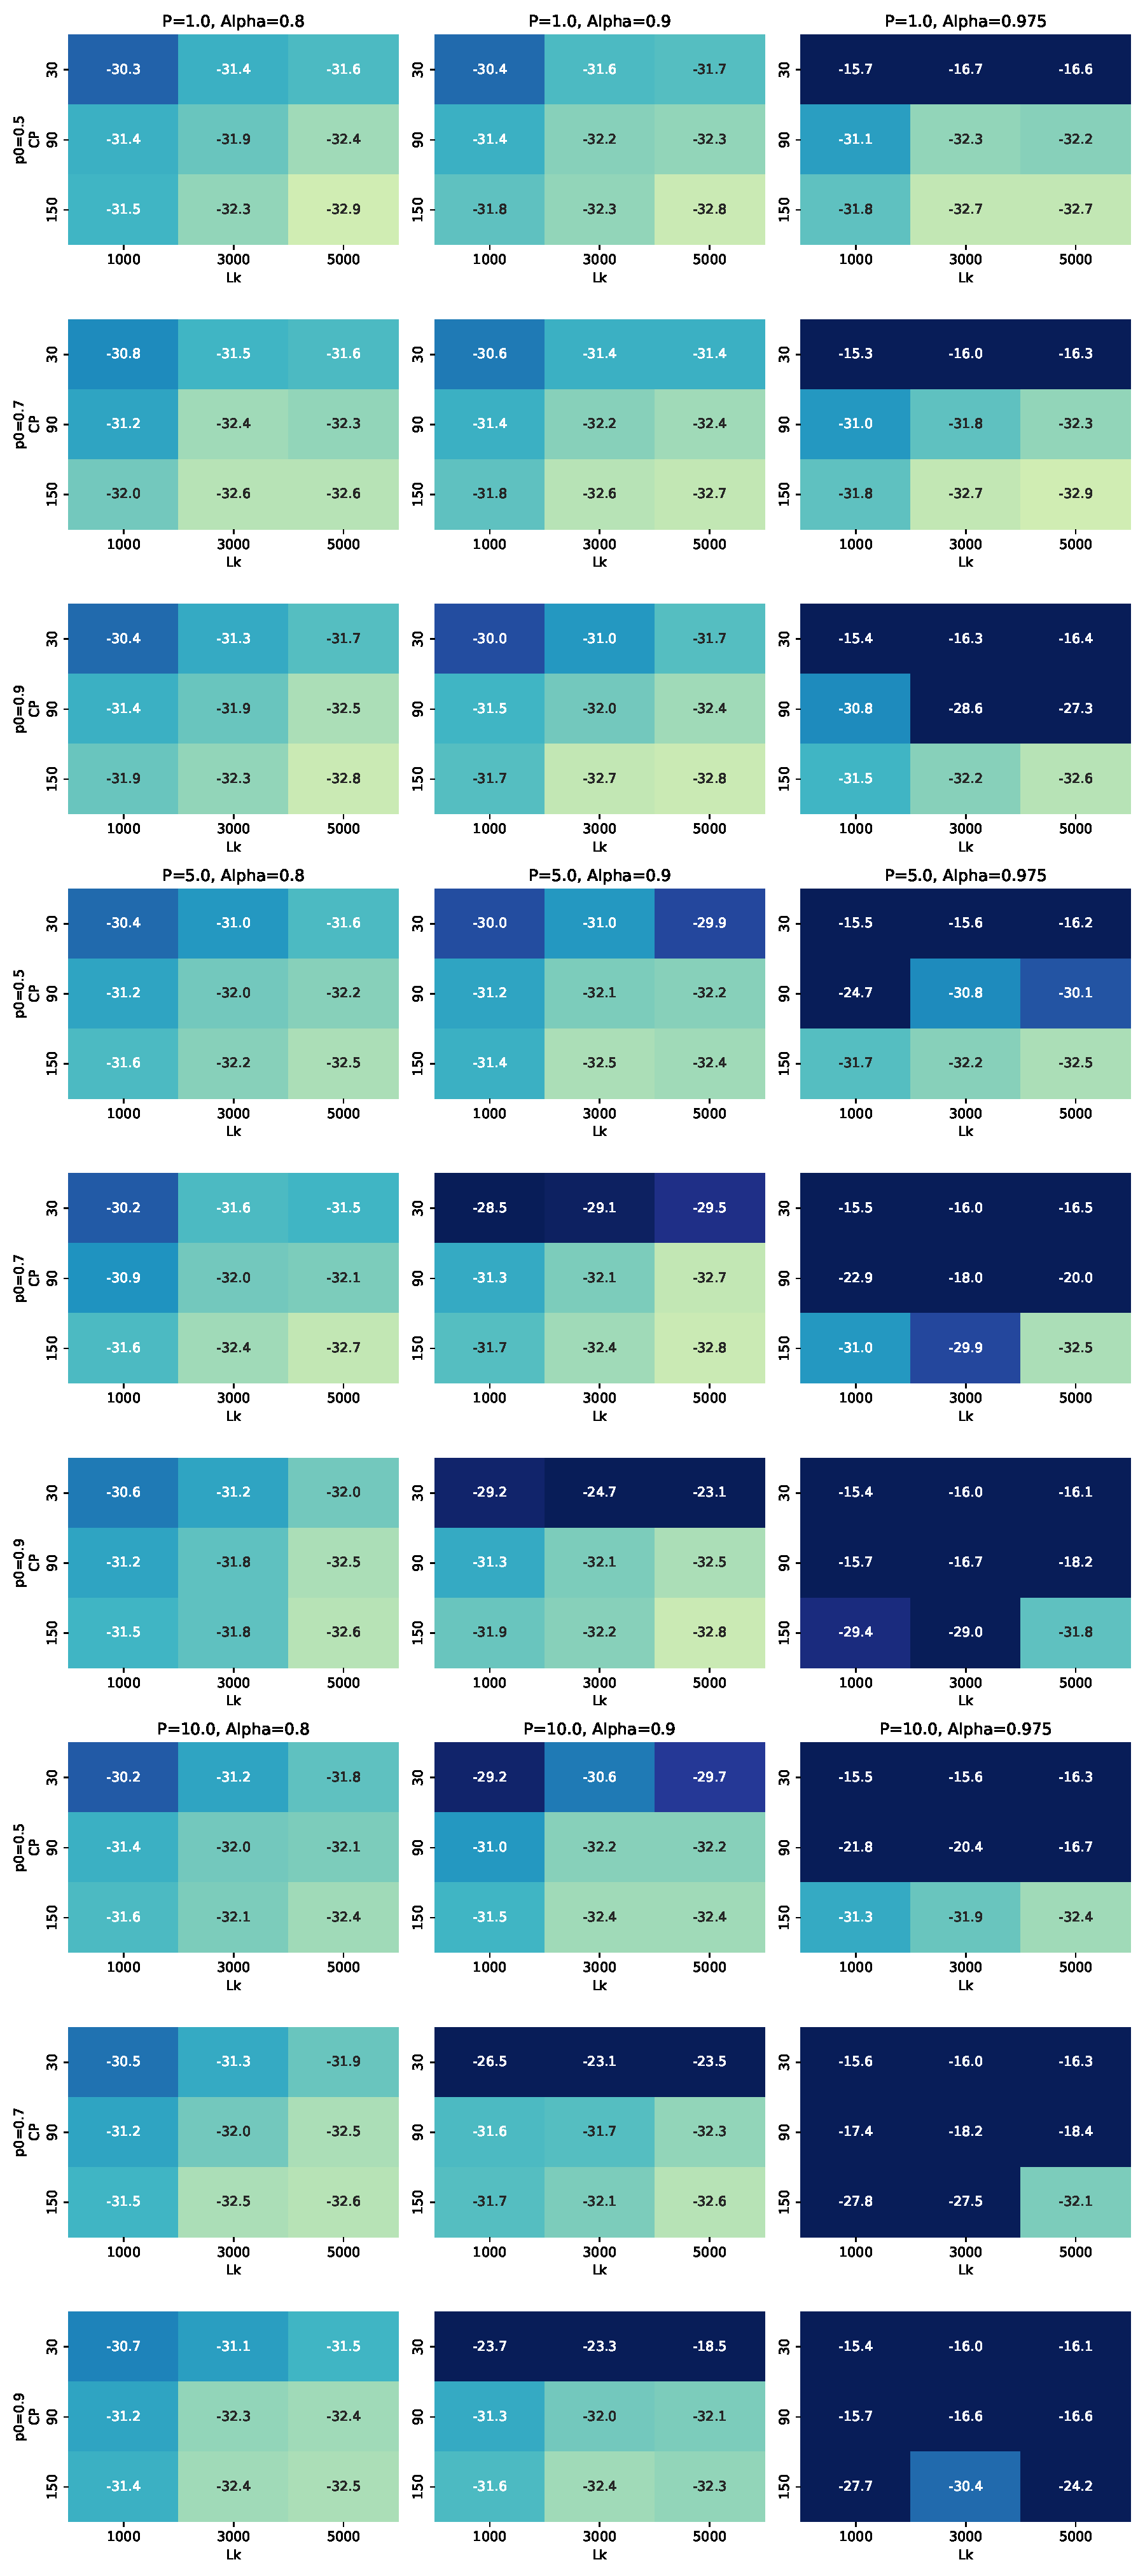
\includegraphics[width = \textwidth]{P2M1_NNGV_objf}
		\caption{Média do mínimo de número de trabalhos}
		\label{fig:P2M1_NNGV_objf}
	\end{subfigure}
	\begin{subfigure}{0.49\textwidth}
	\centering
		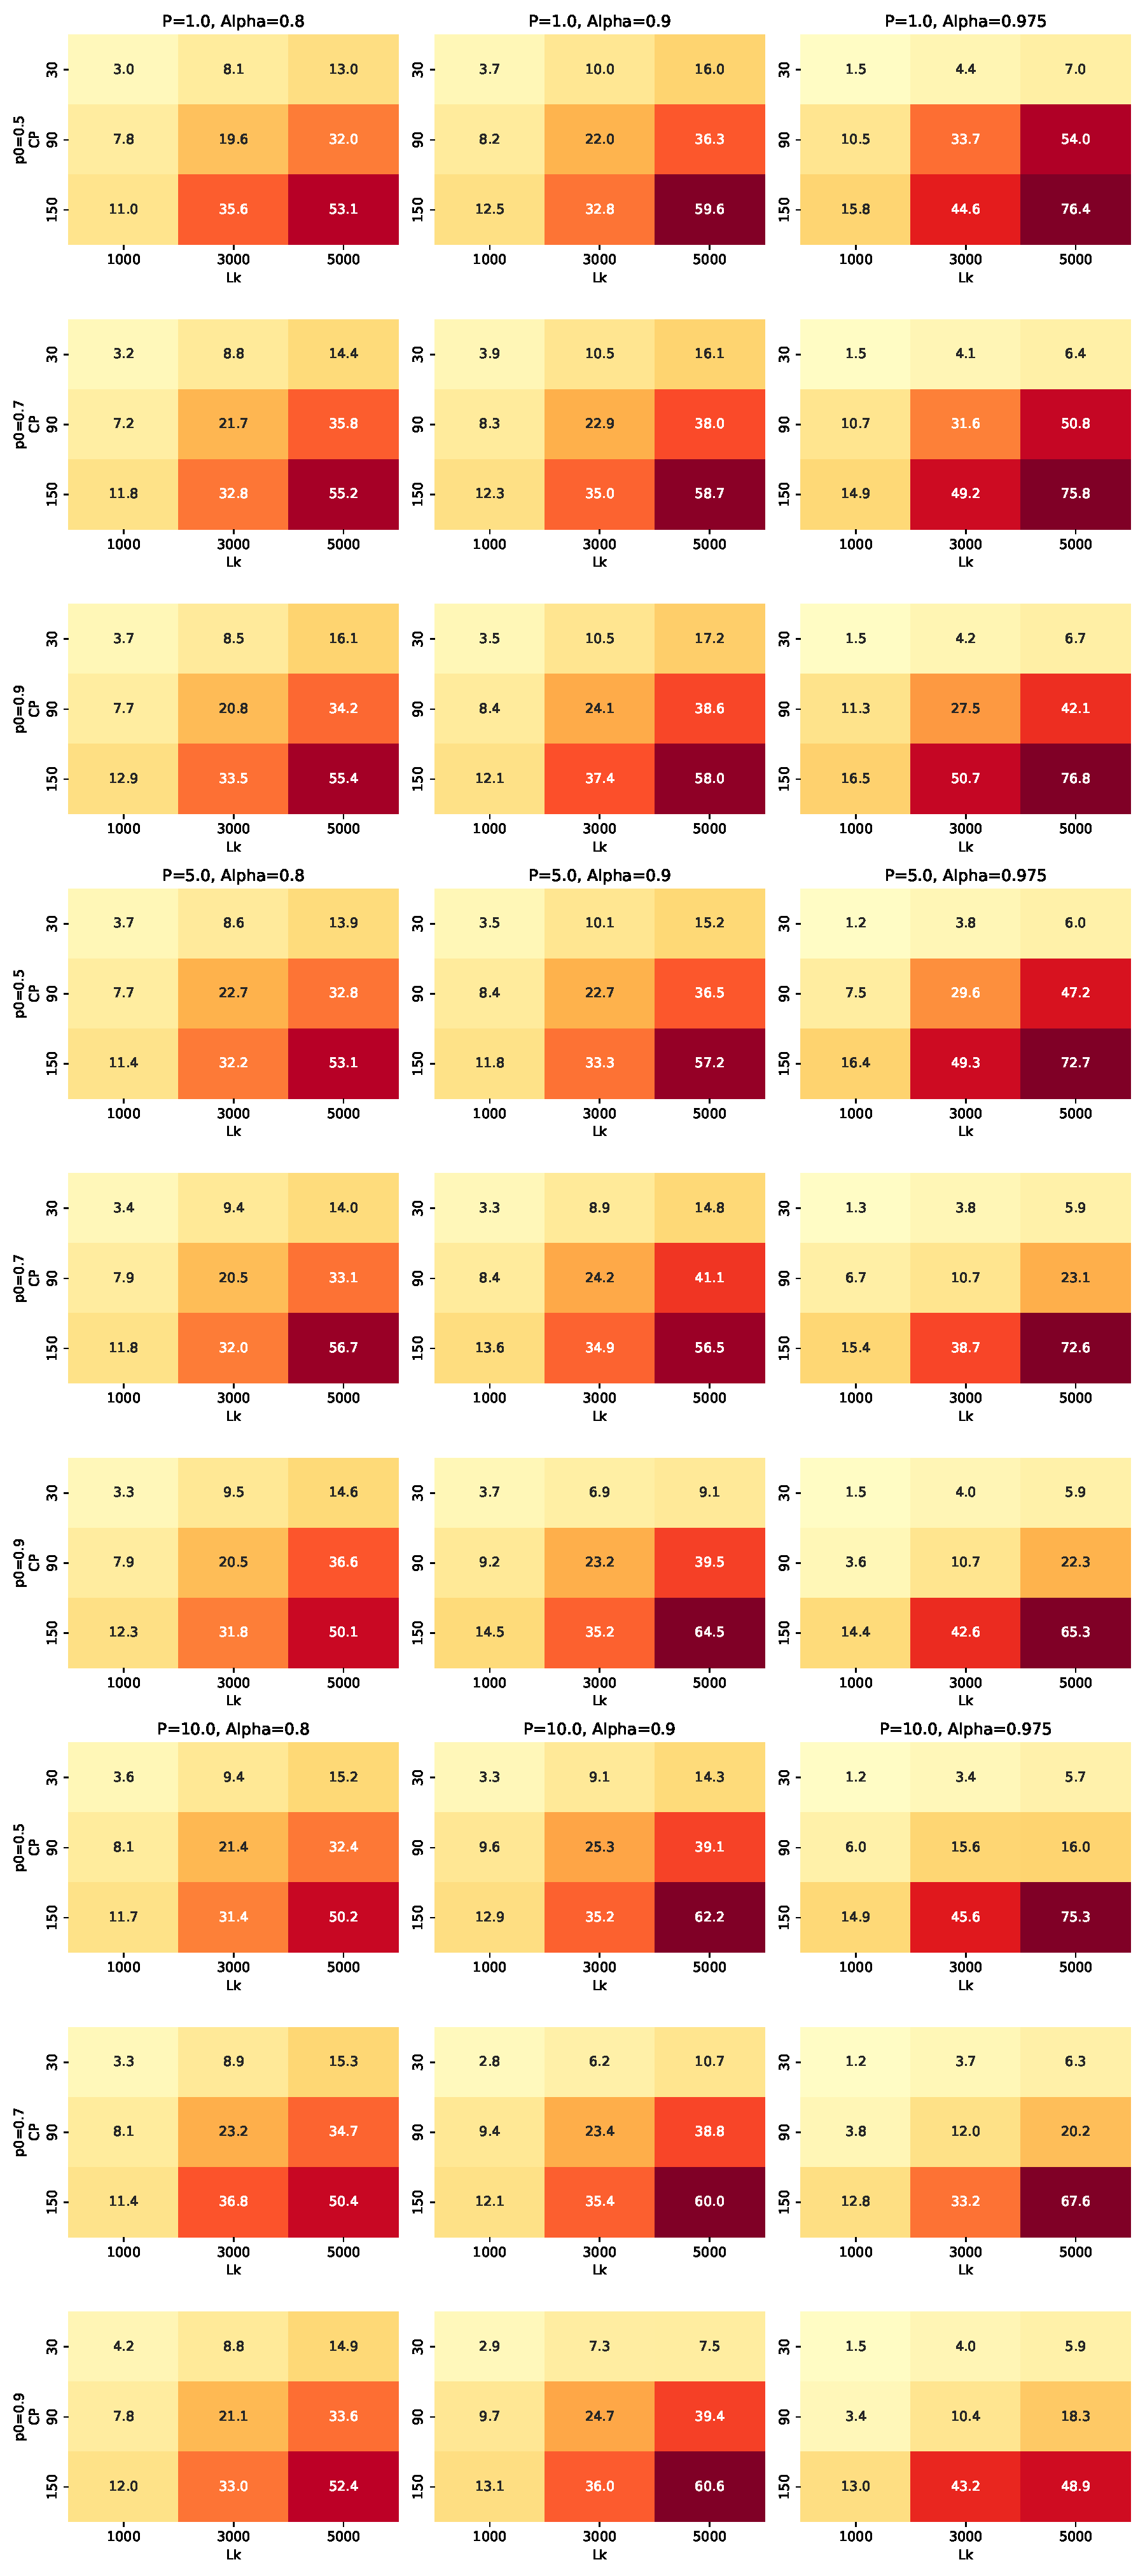
\includegraphics[width = \textwidth]{P2M1_NNGV_time}
		\caption{Média do máximo do tempo de computação}
		\label{fig:P2M1_NNGV_time}
	\end{subfigure}
	\caption{Impacto dos níveis das variáveis sobre o valor da função objetivo e do tempo computacional para o Modelo 1.}
	\label{fig:P2M1_NNGV}
\end{figure}

Com a ajuda da Tabela~\ref{tab:P2M1_NNGV_trabalhos} do Apêndice~\ref{chp:tabelas} pode-se tecer alguns comentários sobre os valores ótimos das variáveis primárias, em relação ao número de exames:
\begin{itemize}
\item $L_{k}$ apresenta efeito linear significativo negativo, o nível a escolher será o alto;
\item $CP$ apresenta efeito linear e quadrático significativo, ambos negativos, o nível a escolher será o alto;
\item $\alpha$ apresenta efeitos lineares e quadráticos significativos, positivo e negativo, respetivamente, o nível a escolher será o baixo;
\item $P$ apresenta efeito linear significativo positivo, o nível a escolher será o baixo.
\item $p_{0}$ apresenta efeito linear significativo positivo, o nível a escolher será o baixo.
\end{itemize}
Relativamente ao tempo, pode-se fazer uma análise semelhante pela Tabela~\ref{tab:P2M1_NNGV_tempo}:
\begin{itemize}
\item $L_{k}$ apresenta efeito linear significativo positivo, o nível a escolher será o baixo;
\item $CP$ apresenta efeito linear significativo positivo, o nível a escolher será o baixo;
\item $\alpha$ apresenta efeitos lineares e quadráticos significativos, ambos positivos, tornando a escolha do nível difícil;
\item $P$ apresenta efeito linear significativo negativo, o nível a escolher será o alto;
\item $p_{0}$ não apresenta efeito linear ou quadrático significativo, o nível a escolher será aquele mais conveniente.
\end{itemize}

De forma a obter uma boa combinação de variáveis utilizou-se uma função a maximizar que utiliza ambas as variáveis dependentes, tal é dada por:\\
$$\frac{n_{exames}^{4}}{tempo^{0,1}}$$

Difere da utilizada no problema anterior porque queremos maximizar o número de exames agendados enquanto se minimiza o tempo necessário, o exponente sobre o número de exames é menor de forma a não sobre-valorizar demais pequenas melhorias da qualidade da solução em troca de aumento excessivo do tempo computacional. Finalmente, definimos que a combinação que maximiza a fórmula é $\{1000; 150; 0,8; 1; 0,7\}$, com o número médio de exames agendados de 32,0 e tempo computacional médio de 11,8 segundos.\\

\subsection{Modelo 2}

De seguida, apresenta-se um novo diagrama de calor contendo os valores da função objetivo e do tempo computacional associados às combinações de níveis provenientes do Modelo 2. As cores do diagrama continuam a ser limitadas com os valores já referidos.\\

Com a análise da Figura~\ref{fig:P2M1_GV} podemos comentar o impacto de cada variável sobre a função objetivo e o tempo computacional. Observamos que, em geral, a qualidade das soluções apresentadas é muito superior para um mesmo tempo computacional. Continuamos a verificar as observações já referidas para o modelo anterior.\\
\begin{figure}[H]
	\centering
	\begin{subfigure}{0.49\textwidth}
	\centering
		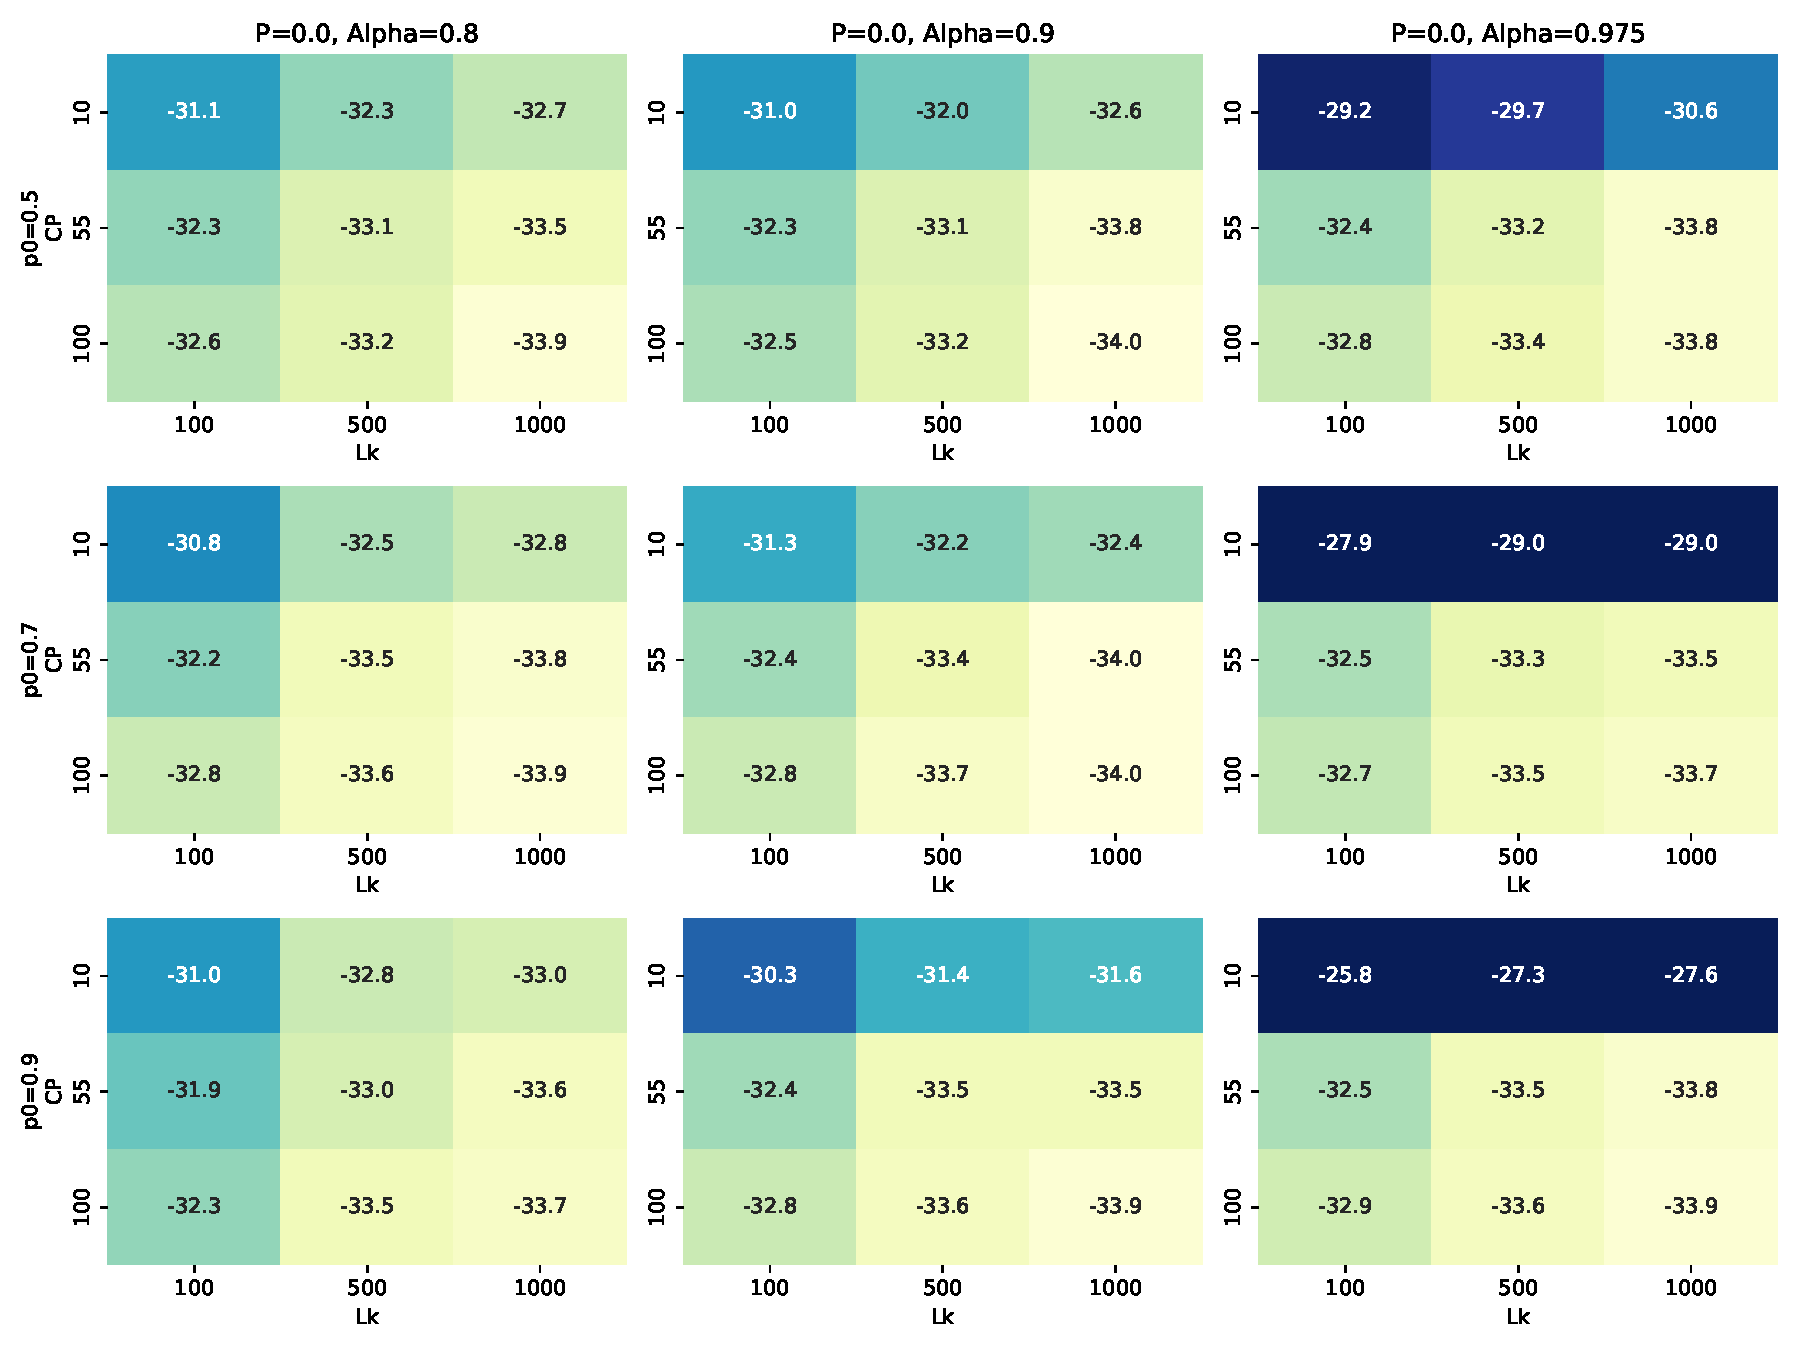
\includegraphics[width = \textwidth]{P2M1_GV_objf}
		\caption{Média do mínimo de número de trabalhos}
		\label{fig:P2M1_GV_objf}
	\end{subfigure}
	\begin{subfigure}{0.49\textwidth}
	\centering
		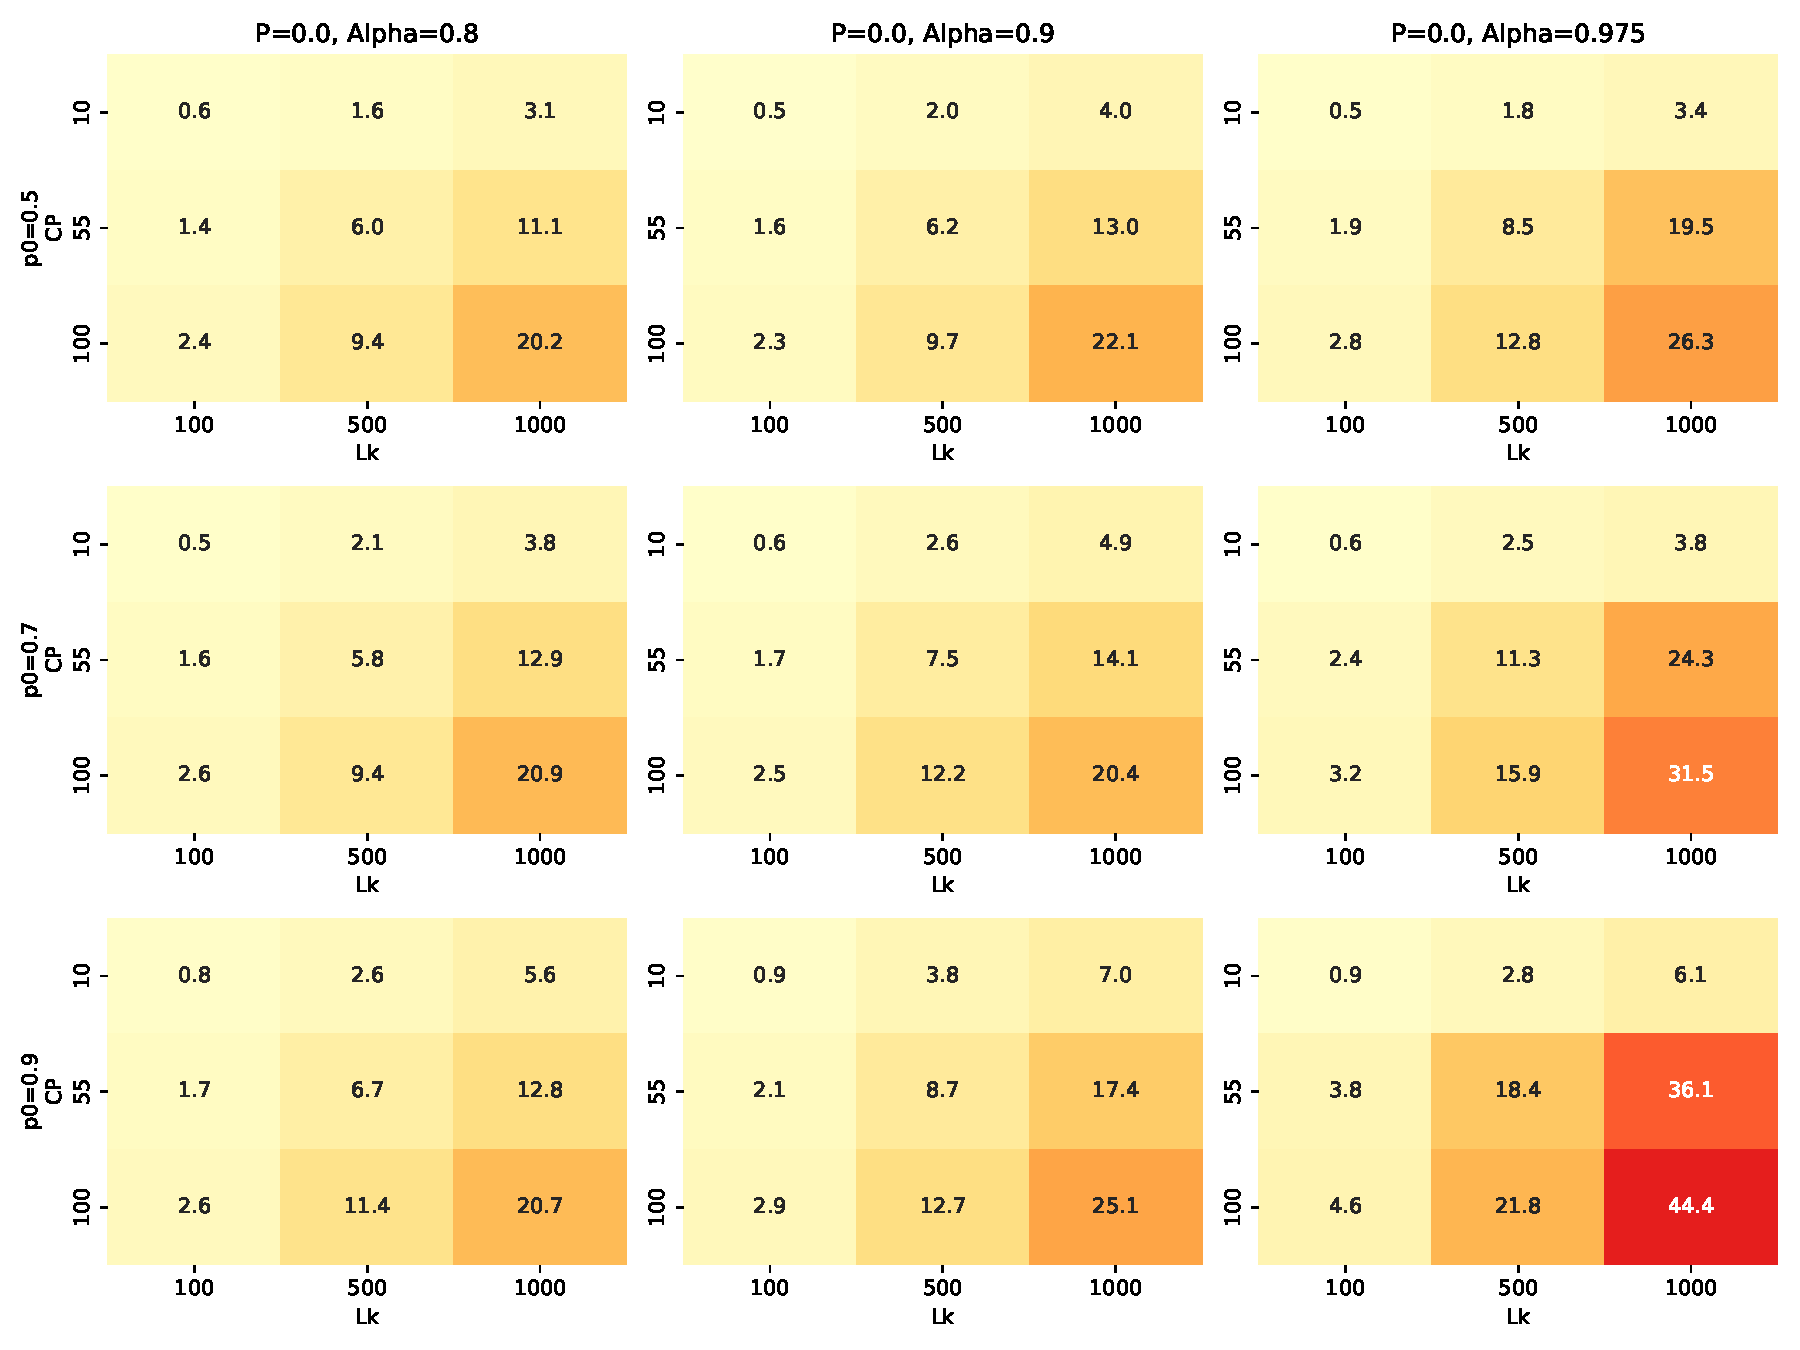
\includegraphics[width = \textwidth]{P2M1_GV_time}
		\caption{Média do máximo do tempo de computação}
		\label{fig:P2M1_GV_time}
	\end{subfigure}
	\caption{Impacto dos níveis das variáveis sobre o valor da função objetivo e do tempo computacional para o Modelo 2.}
	\label{fig:P2M1_GV}
\end{figure}

Com a Tabela~\ref{tab:P2M1_GV_trabalhos} pode-se tecer comentários mais concretos relativamente ao impacto de cada variável sobre a qualidade da solução:
\begin{itemize}
\item $L_{k}$ apresenta efeito linear e quadrático significativos, ambos negativos, o nível a escolher será o alto;
\item $CP$ apresenta efeito linear e quadrático significativos, ambos negativos, o nível a escolher será o alto;
\item $\alpha$ apresenta efeitos lineares e quadráticos significativos, positivo e negativo, respetivamente, o nível a escolher será o baixo;
\item $p_{0}$ apresenta efeito linear significativo positivo, o nível a escolher será o baixo.
\end{itemize}
Relativamente ao tempo computacional, utiliza-se a tabela~\ref{tab:P2M1_GV_tempo}:
\begin{itemize}
\item $L_{k}$ apresenta efeito linear significativo positivo, o nível a escolher será o baixo;
\item $CP$ apresenta efeito linear e quadrático significativo, ambos positivos, a escolher torna-se difícil, mas intuitivamente devemos escolher o nível baixo;
\item $\alpha$ apresenta efeito linear e quadrático significativos, positivo e negativo, respetivamente, o nível a escolher será o baixo;
\item $p_{0}$ apresenta efeito linear significante positivo, o nível a escolher será o baixo.
\end{itemize}

A combinação que maximiza a fórmula já descrita é $\{100; 100; 0,9; 0; 0,7\}$, com o número médio de exames agendados de 32,8 e tempo computacional médio de 2,5 segundos.\\

\subsection{Modelo 3}

Um novo diagrama de calor será apresentado, na Figura~\ref{fig:P2M2_GV_alt}, desta vez referente ao Modelo 3, contendo as várias combinação de níveis referentes a este modelo. A faixa de cores continua a ser limitada como de antes.

\begin{figure}[h]
	\centering
	\begin{subfigure}{0.49\textwidth}
	\centering
		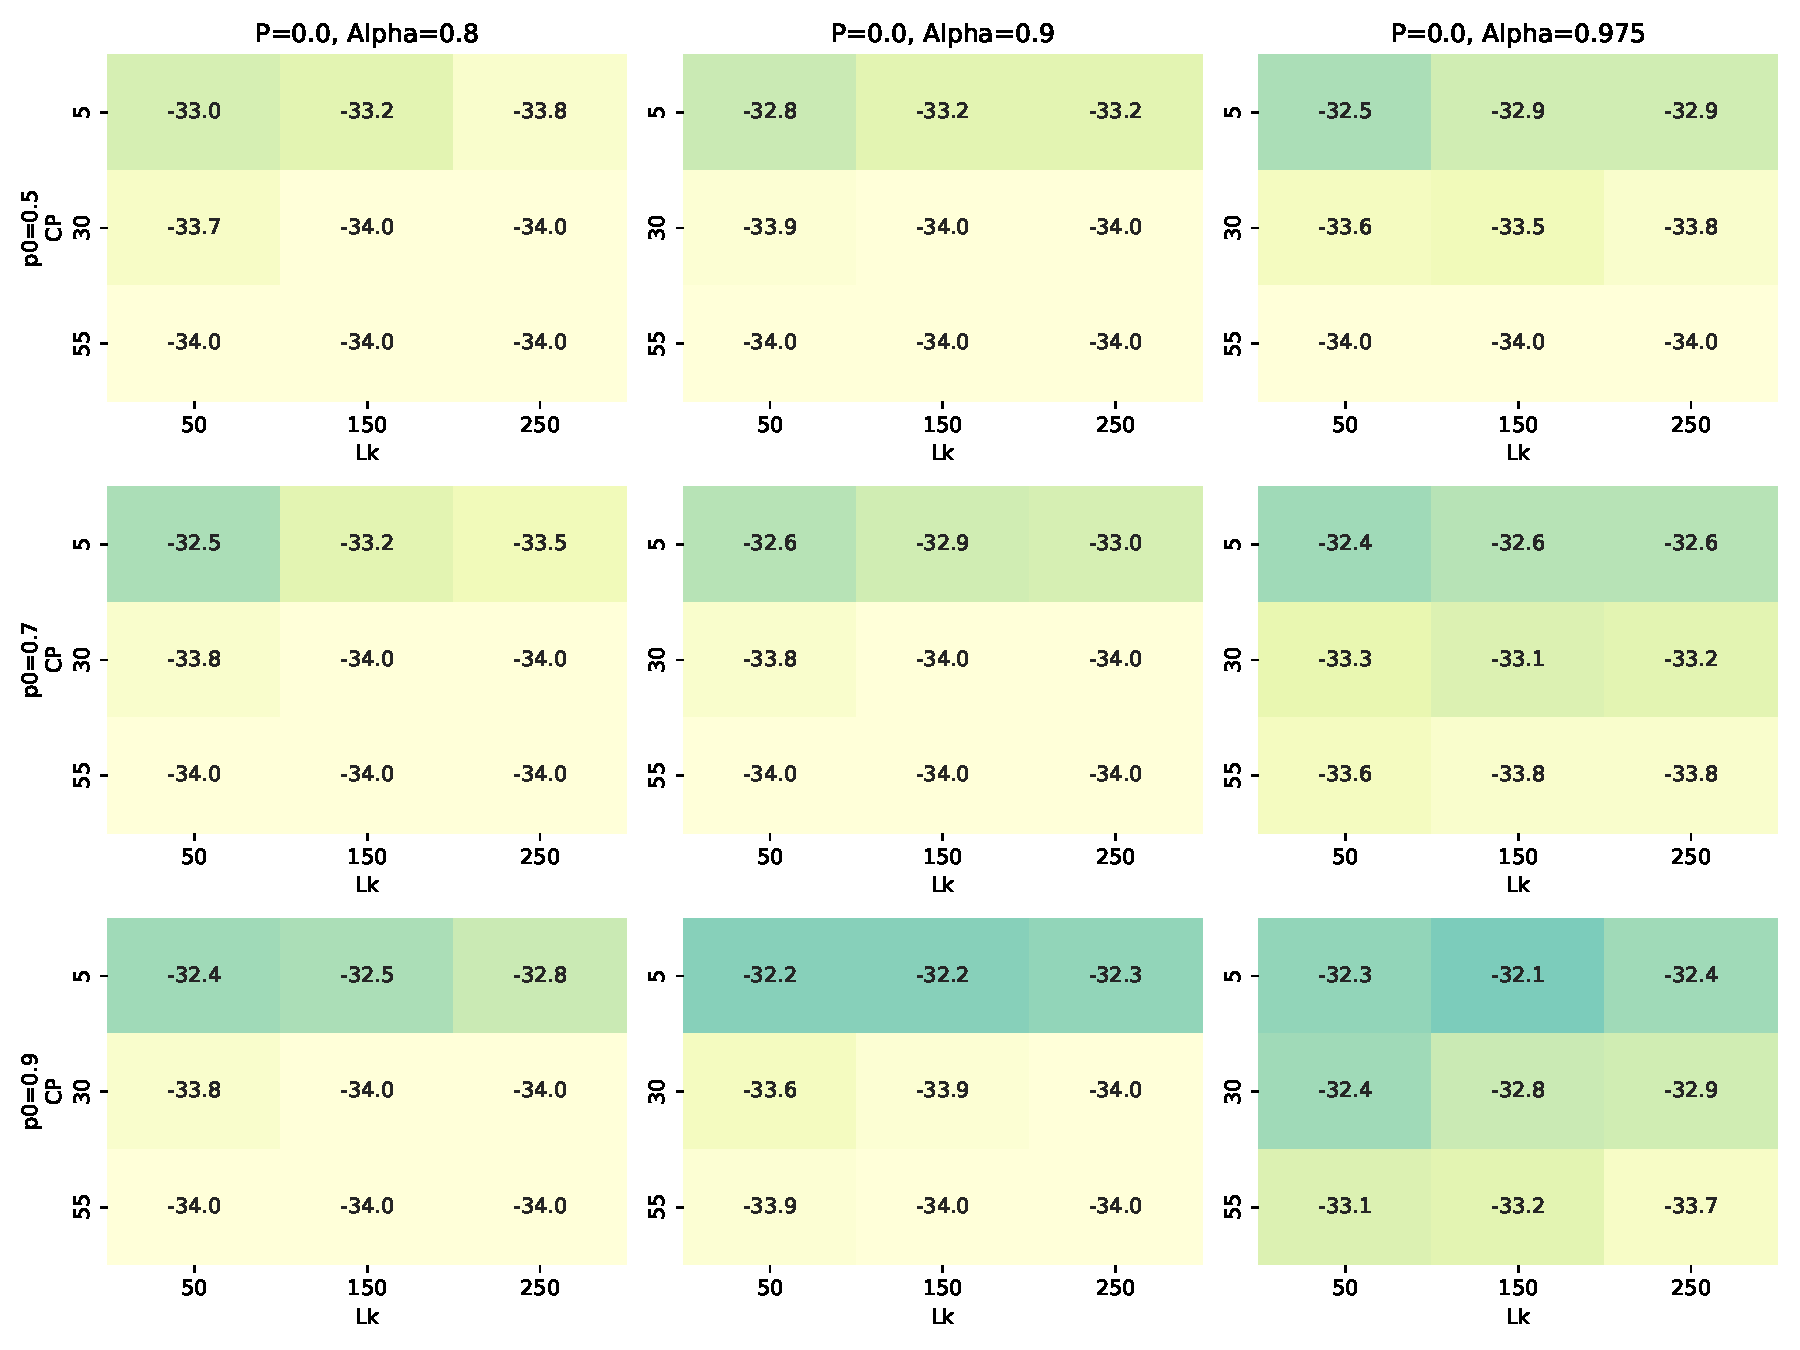
\includegraphics[width = \textwidth]{P2M2_GV_alt_objf}
		\caption{Média do mínimo de número de trabalhos}
		\label{fig:P2M2_GV_alt_objf}
	\end{subfigure}
	\begin{subfigure}{0.49\textwidth}
	\centering
		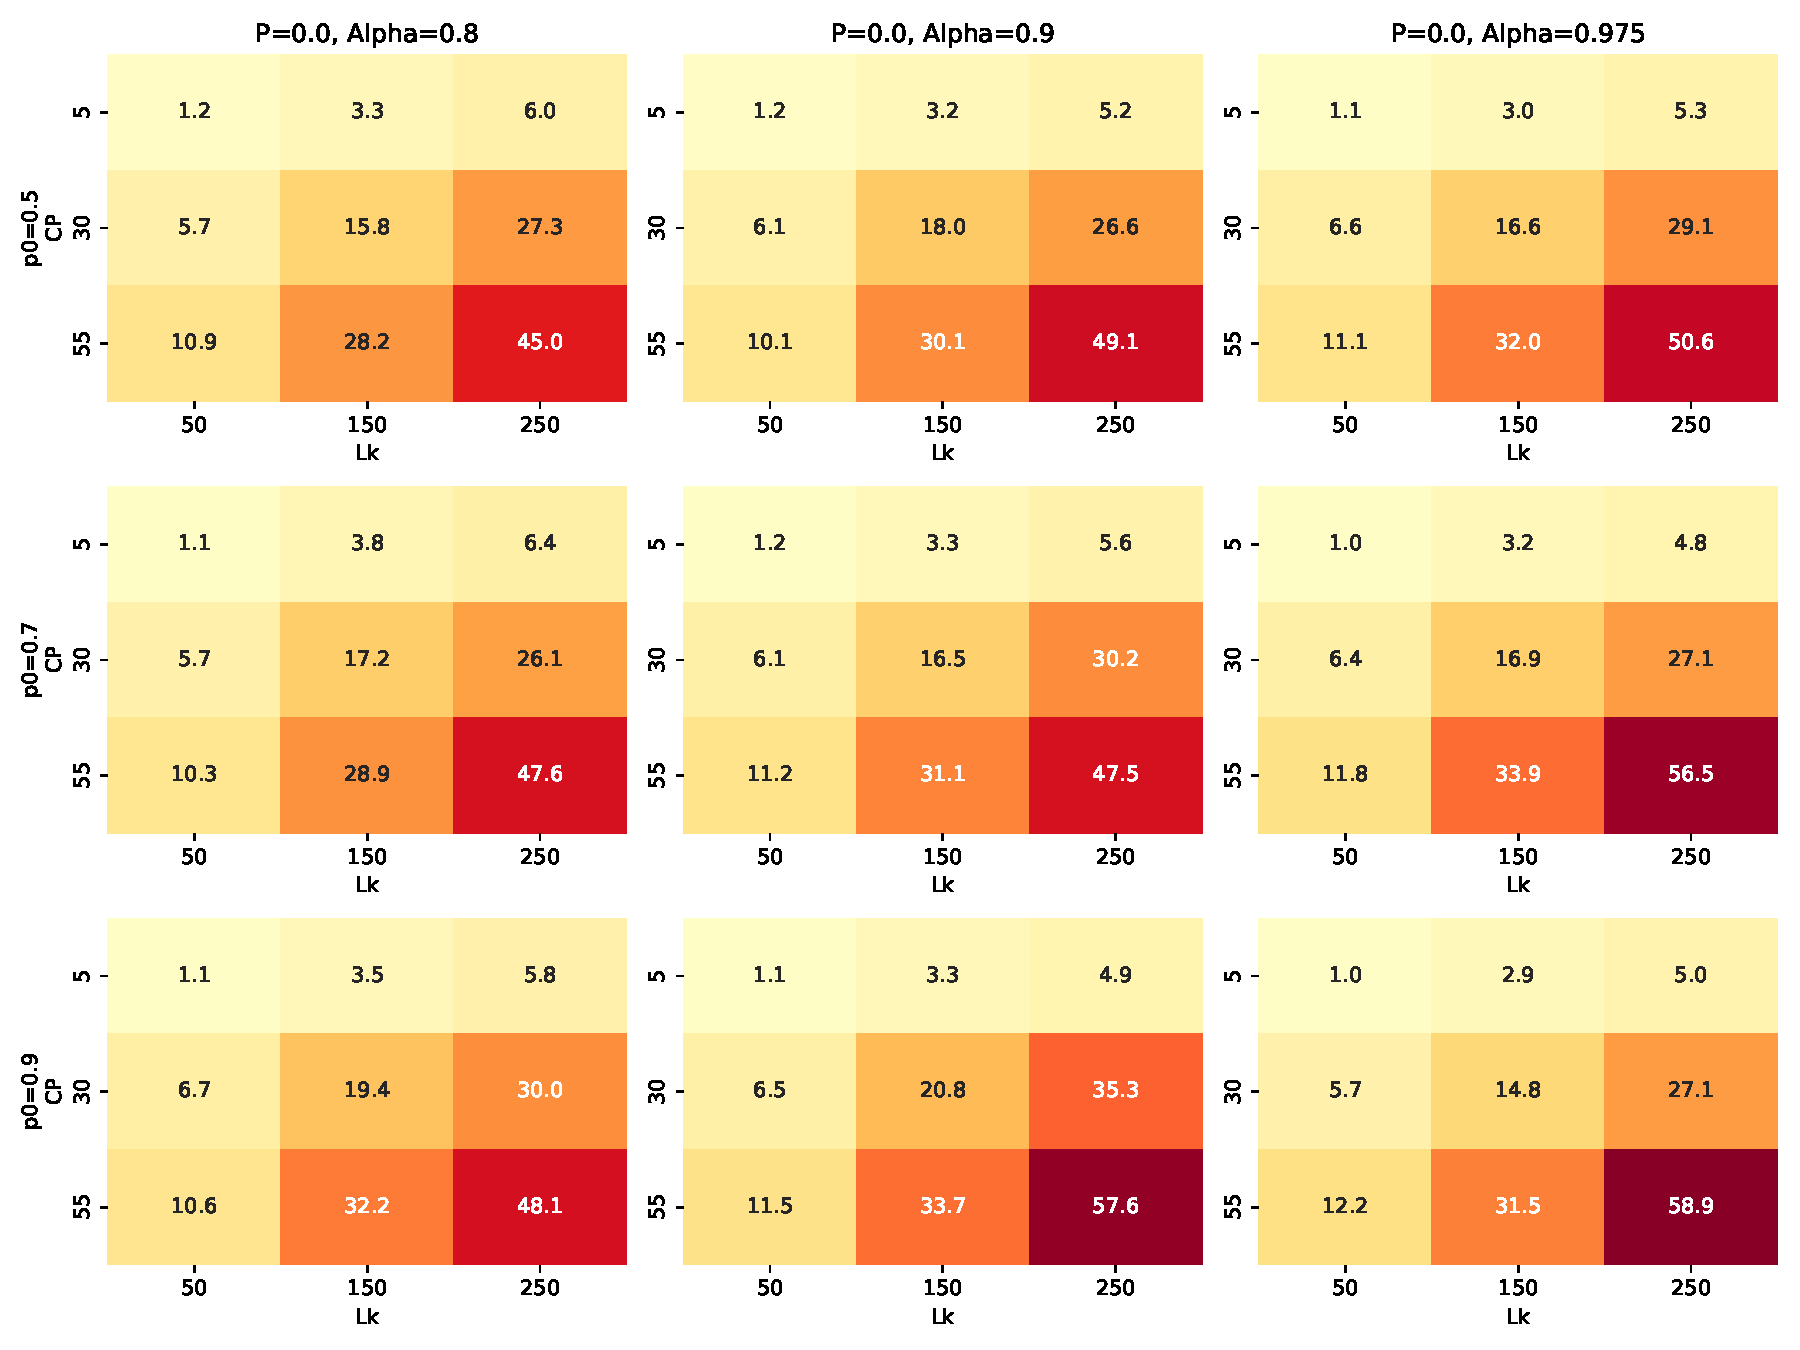
\includegraphics[width = \textwidth]{P2M2_GV_alt_time}
		\caption{Média do máximo do tempo de computação}
		\label{fig:P2M2_GV_alt_time}
	\end{subfigure}
	\caption{Impacto dos níveis das variáveis sobre o valor da função objetivo e do tempo computacional para o Modelo 3.}
	\label{fig:P2M2_GV_alt}
\end{figure}

Através da análise da figura~\ref{fig:P2M2_GV_alt} observa-se que este modelo apresenta melhores soluções para o mesmo tempo computacional. Qualquer outro comentário será repetido dos já feitos.\\

Pela tabela~\ref{tab:P2M2_GV_trabalhos} pode-se perceber o efeito principal de cada variável sobre a qualidade da solução.
\begin{itemize}
\item $L_{k}$ apresenta efeito linear significativo negativo, o nível a escolher será o alto;
\item $CP$ apresenta efeito linear e quadrático significativos, ambos negativos, o nível a escolher será o alto;
\item $\alpha$ apresenta efeito linear e quadrático significativos, positivo e negativo, respetivamente, o nível a escolher será o baixo;
\item $p_{0}$ apresenta efeito linear significativo positivo, o nível a escolher será o baixo.
\end{itemize}
Pela tabela~\ref{tab:P2M2_GV_tempo} pode-se perceber o efeito principal de cada variável sobre o tempo computacional.
\begin{itemize}
\item $L_{k}$ apresenta efeito linear significativo positivo, o nível a escolher será o baixo;
\item $CP$ apresenta efeito linear significativo positivo, o nível a escolher será o baixo;
\item $\alpha$ apresenta efeito linear significativo positivo, o nível a escolher será o baixo;
\item $p_{0}$ apresenta efeito linear significativo positivo, o nível a escolher será o baixo;
\end{itemize}

A combinação que maximiza a fórmula já descrita é $\{50; 5; 0,8; 0; 0,5\}$, com o número médio de exames agendados de 33,0 e tempo computacional médio de 1,2 segundos.\\

\subsection{Comparação entre modelos}

De seguida são apresentados, para cada dia da semana, os exames que podem ser realizados. Para cada um dos dias, utilizou-se o dobro do número de exames relativamente ao problema anterior. Por sua vez, $T_{\max}$ será o melhor valor de \textit{makespan} encontrado. O Modelo 3 \textit{ND} e \textit{END} têm o seu instante de começo definido pelos Algoritmos~\ref{algo:non-delay-TT_P2} e~\ref{algo:enh-non-delay-TT_P2}, respetivamente. Cada dia será resolvido utilizando cada um dos modelos com as variáveis já mencionadas.\\

\begin{itemize}
\item Segunda-feira: 6 cintigrafia tiroideia, 10 cintigrafia pulmonar de ventilação/inalação + perfusão, 20 cintigrafia miocárdica de perfusão em repouso, 2 cintigrafia das glândulas salivares, 20 PET - estudo corpo inteiro com FDG;
\item Terça-feira: 4 cintigrafia tiroideia, 20 cintigrafia óssea corpo inteiro, 2 cintigrafia para amiloidose cardíaca, 2 linfocintigrafia para detecção de gânglio sentinela, 4 cintigrafia pulmonar de ventilação/inalação + perfusão, 20 PET - estudo corpo inteiro com FDG;
\item Quarta-feira: 4 cintigrafia tiroideia, 4 linfocintigrafia para detecção de gânglio sentinela, 12 cintigrafia das paratiroideias, 2 tomografia cerebral com 123I-ioflupano, 6 cintigrafia pulmonar de ventilação/inalação + perfusão, 16 PET - estudo corpo inteiro com FDG;
\item Quinta-feira: 12 linfocintigrafia para detecção de gânglio sentinela, 24 cintigrafia miocárdica de perfusão em esforço/stress farmacológico, 2 tomografia cerebral com 123I-ioflupano, 4 cintigrafia miocárdica de perfusão em repouso, 20 PET - estudo corpo inteiro com FDG.
\end{itemize}

Com a Tabela~\ref{tab:P2_dias} pode-se comparar os modelos na resolução dos quatro dias apresentados, utilizou-se a melhor solução proveniente do modelo $MILP-\delta$. Observamos que, até com 8 horas de tempo computacional alocado, nem sempre temos a garantia do valor ótimo.\\
Verificamos de novo que o Modelo 1 é superado pelo Modelo 2 e 3 em qualidade da solução e em tempo computacional necessário. Por sua vez, o Modelo 3 com as suas variantes apresenta soluções marginalmente melhores que o modelo 2, em tempo computacional comparável. Como seria de esperar, todos os modelos apresentam soluções melhores que a heurística NEH.\\
\begin{landscape}
\begin{table}[H]
\caption{Resultados provenientes dos três modelos em relação aos problemas de cada dia da semana.}
\label{tab:P2_dias}
\setlength{\tabcolsep}{2pt} % smaller horizontal padding
\begin{tabular}{llccccccccccccccc}
\multirow{2}{*}{Dia} & \multicolumn{1}{l|}{\multirow{2}{*}{$BKS$}} & \multicolumn{3}{c|}{\textit{MILP-$\delta$}}                                & \multicolumn{4}{c|}{Modelo 1}                                                                & \multicolumn{4}{c|}{Modelo 2}                                                                         & \multicolumn{4}{c}{Modelo 3 \textit{LS}}                                       \\
                     & \multicolumn{1}{l|}{}                       & $BRPD$               & $BBRPD$              & \multicolumn{1}{c|}{$TCT$}   & $BRPD$                     & $ARPD$               & $TCT$                & \multicolumn{1}{c|}{$ACT$} & $BRPD$                     & $ARPD$               & $TCT$                & \multicolumn{1}{c|}{$ACT$} & $BRPD$                     & $ARPD$               & $TCT$                & $ACT$                \\ \hline
Segunda-Feira        & \multicolumn{1}{l|}{34}                     & 0,00                 & -8,82                & \multicolumn{1}{c|}{28800}   & 2,94                       & 5,88                 & 84,1                 & \multicolumn{1}{c|}{11,8}  & 2,94                       & 3,53                 & 18,7                 & \multicolumn{1}{c|}{2,5}   & 2,94                       & 2,94                 & 10,5                 & 1,2                  \\
Terça-Feira          & \multicolumn{1}{l|}{34}                     & 0,00                 & 0,00                 & \multicolumn{1}{c|}{2555}    & 5,88                       & 6,76                 & 89,5                 & \multicolumn{1}{c|}{11,9}  & 0,00                       & 3,82                 & 18,5                 & \multicolumn{1}{c|}{2,4}   & 2,94                       & 2,94                 & 19,5                 & 2,5                  \\
Quarta-Feira         & \multicolumn{1}{l|}{33}                     & 0,00                 & 0,00                 & \multicolumn{1}{c|}{74}      & 6,06                       & 6,06                 & 83,8                 & \multicolumn{1}{c|}{10,8}  & 3,03                       & 5,15                 & 27,1                 & \multicolumn{1}{c|}{3,4}   & 0,00                       & 2,12                 & 15,0                 & 1,6                  \\
Quinta-Feira         & \multicolumn{1}{l|}{36}                     & 0,00                 & -11,11               & \multicolumn{1}{c|}{28800}   & 8,33                       & 8,61                 & 92,3                 & \multicolumn{1}{c|}{12,9}  & 2,78                       & 5,00                 & 24,9                 & \multicolumn{1}{c|}{3,3}   & 0,00                       & 2,78                 & 40,3                 & 5,9                  \\ \hline
Média                & \multicolumn{1}{l|}{}                       & 0,00                 & -4,98                & \multicolumn{1}{c|}{15057,3} & 5,80                       & 6,83                 & 87,4                 & \multicolumn{1}{c|}{11,9}  & 2,19                       & 4,38                 & 22,3                 & \multicolumn{1}{c|}{2,9}   & 1,47                       & 2,70                 & 21,3                 & 2,8                  \\
                     &                                             & \multicolumn{1}{l}{} & \multicolumn{1}{l}{} & \multicolumn{1}{l}{}         & \multicolumn{1}{l}{}       & \multicolumn{1}{l}{} & \multicolumn{1}{l}{} & \multicolumn{1}{l}{}       & \multicolumn{1}{l}{}       & \multicolumn{1}{l}{} & \multicolumn{1}{l}{} & \multicolumn{1}{l}{}       & \multicolumn{1}{l}{}       & \multicolumn{1}{l}{} & \multicolumn{1}{l}{} & \multicolumn{1}{l}{} \\
                     &                                             & \multicolumn{1}{l}{} & \multicolumn{1}{l}{} & \multicolumn{1}{l}{}         & \multicolumn{1}{l}{}       & \multicolumn{1}{l}{} & \multicolumn{1}{l}{} & \multicolumn{1}{l}{}       & \multicolumn{1}{l}{}       & \multicolumn{1}{l}{} & \multicolumn{1}{l}{} & \multicolumn{1}{l}{}       & \multicolumn{1}{l}{}       & \multicolumn{1}{l}{} & \multicolumn{1}{l}{} & \multicolumn{1}{l}{} \\
\multirow{2}{*}{Dia} & \multicolumn{1}{l|}{\multirow{2}{*}{$BKS$}} & \multicolumn{4}{c|}{Modelo 3 \textit{ELS}}                                             & \multicolumn{4}{c|}{Modelo 3 \textit{ND}}                                            & \multicolumn{4}{c|}{Modelo 3 \textit{END}}                                           & \multicolumn{2}{c}{NEH}                     &                      \\
                     & \multicolumn{1}{l|}{}                       & $BRPD$               & $ARPD$               & $TCT$                        & \multicolumn{1}{c|}{$ACT$} & $BRPD$               & $ARPD$               & $TCT$                      & \multicolumn{1}{c|}{$ACT$} & $BRPD$               & $ARPD$               & $TCT$                      & \multicolumn{1}{c|}{$ACT$} & $BRPD$               & $TCT$                &                      \\ \cline{1-16}
Segunda-Feira        & \multicolumn{1}{l|}{34}                     & 0,00                 & 2,65                 & 21,9                         & \multicolumn{1}{c|}{2,8}   & 2,94                 & 5,00                 & 5,6                        & \multicolumn{1}{c|}{0,8}   & 2,94                 & 5,59                 & 16,6                       & \multicolumn{1}{c|}{2,2}   & 14,71                & 2,8                  &                      \\
Terça-Feira          & \multicolumn{1}{l|}{34}                     & 0,00                 & 1,76                 & 18                           & \multicolumn{1}{c|}{2,3}   & 0,00                 & 3,53                 & 6,1                        & \multicolumn{1}{c|}{0,9}   & 0,00                 & 4,41                 & 16,2                       & \multicolumn{1}{c|}{2,3}   & 8,82                 & 3,2                  &                      \\
Quarta-Feira         & \multicolumn{1}{l|}{33}                     & 0,00                 & 1,52                 & 14,6                         & \multicolumn{1}{c|}{1,7}   & 3,03                 & 3,33                 & 5,7                        & \multicolumn{1}{c|}{0,6}   & 3,03                 & 3,33                 & 12,9                       & \multicolumn{1}{c|}{1,9}   & 6,06                 & 1,6                  &                      \\
Quinta-Feira         & \multicolumn{1}{l|}{36}                     & 0,00                 & 3,33                 & 36,5                         & \multicolumn{1}{c|}{5,2}   & 2,78                 & 6,67                 & 8,1                        & \multicolumn{1}{c|}{1,1}   & 2,78                 & 5,56                 & 20,3                       & \multicolumn{1}{c|}{2,9}   & 19,44                & 5,5                  &                      \\ \cline{1-16}
Média                & \multicolumn{1}{l|}{}                       & 0,00                 & 2,32                 & 22,75                        & \multicolumn{1}{c|}{3,00}  & 2,19                 & 4,63                 & 6,38                       & \multicolumn{1}{c|}{0,85}  & 2,19                 & 4,72                 & 16,50                      & \multicolumn{1}{c|}{2,33}  & 12,26                & 3,3                  &                     
\end{tabular}
\end{table}
\end{landscape}

\subsection{Comparação com instâncias de \textit{benchmark}}

De seguida são apresentados os resultados provenientes das instâncias já discutidas, para cada uma utilizou-se o dobro dos trabalhos e utilizou-se $T_{\max}$ como o melhor valor de \textit{makespan} já reportado na literatura, ou seja, o valor $BKS$ do problema anterior.\\

Para a tabela~\ref{tab:P2_instan} compara-se a formulação \textit{MILP-$\delta$}, os três modelos, e a heurística NEH. Para a formulação \textit{MILP-$\delta$} apenas se alocou 2 horas, verifica-se que não apresenta soluções ótimas porque $BRPD$ é constantemente superior a 0, ao mesmo tempo é difícil saber se $BKS$ se encontra próximo do valor ótimo devido aos valores alto de $BBRPD$. Assim o valor de $BKS$ reportado é o melhor valor alcançado entre a formulação \textit{MILP-$\delta$} e os modelos.\\

O Modelo 3 apresenta-se como a escolha óbvia para a resolução destas instâncias, contudo a diferença verificada entre as variantes deste modelo torna a escolha difícil de se fazer. Mesmo assim todas estas apresentam boas soluções com tempo computacional inferior à dos Modelos 1 e 2. A heurística NEH apresenta soluções semelhantes à média do Modelo 1, fazendo-o com tempo computacional muito inferior.\\

Outra vez, apesar destes modelos não terem sido desenhados para resolver as instâncias aqui apresentadas, é possível fazer uma comparação entre os vários modelos utilizando as Tabelas~\ref{tab:P2_hipothesis_BRPD},~\ref{tab:P2_hipothesis_ARPD},~\ref{tab:P2_hipothesis_TCT},~\ref{tab:P2_hipothesis_ACT}. Em termos de qualidade dos resultados, para um nível de significância de 5\%, não se pode rejeitar a hipótese nula de que o Modelo 3 com os vários algoritmos de \textit{timetabling} apresentam distribuição igual. Desta forma não se pode averiguar qual destes modelos é o melhor. Entre o Modelo 3 e os restantes, como a diferença entre as distribuições já é significante, pode-se admitir que o Modelo 3 é o melhor.\\
\begin{landscape}
\begin{table}[H]
\caption{Resultados provenientes dos três modelos em relação às pequenas instâncias apresentadas em Sundar et al.~\cite{sundarHybridArtificialBee2017}.}
\label{tab:P2_instan}
\setlength{\tabcolsep}{3pt} % smaller horizontal padding
\begin{tabular}{ll|ccc|cccc|cccc|cccc}
\multirow{2}{*}{Instância} & \multirow{2}{*}{$BKS$} & \multicolumn{3}{c|}{\textit{MILP-$\delta$}}  & \multicolumn{4}{c|}{Modelo 1}   & \multicolumn{4}{c|}{Modelo 2}    & \multicolumn{4}{c}{Modelo 3 \textit{LS}} \\
                           &                        & $BRPD$ & $BBRPD$ & $TCT$   & $BRPD$ & $ARPD$ & $TCT$ & $ACT$ & $BRPD$ & $ARPD$ & $TCT$  & $ACT$ & $BRPD$        & $ARPD$        & $TCT$       & $ACT$       \\ \hline
Ft06                       & 7                      & 0,00   & 0,00    & 1       & 14,29  & 14,29  & 40,1  & 4,8   & 14,29  & 14,29  & 5,3    & 0,6   & 0,00          & 0,00          & 2,7         & 0,2         \\
La01                       & 11                     & 9,09   & -36,36  & 7200    & 9,09   & 9,09   & 64,8  & 8,5   & 0,00   & 8,18   & 27,3   & 3,8   & 0,00          & 0,00          & 5,0         & 0,7         \\
La02                       & 12                     & 8,33   & -25,00  & 7200    & 8,33   & 17,50  & 67,2  & 9,5   & 0,00   & 10,00  & 26,3   & 3,4   & 0,00          & 6,67          & 4,7         & 0,6         \\
La03                       & 11                     & 0,00   & -36,36  & 7200    & 0,00   & 10,00  & 54,1  & 8,7   & 0,00   & 7,27   & 24,7   & 3,4   & 0,00          & 0,00          & 4,1         & 0,6         \\
La04                       & 11                     & 9,09   & -36,36  & 7200    & 9,09   & 14,55  & 63,8  & 9,0   & 0,00   & 12,73  & 26,2   & 3,3   & 0,00          & 2,73          & 4,1         & 0,6         \\
La05                       & 11                     & 9,09   & -27,27  & 7200    & 9,09   & 17,27  & 57,3  & 7,7   & 9,09   & 10,91  & 20,0   & 2,4   & 9,09          & 9,09          & 3,7         & 0,5         \\
Ft10                       & 12                     & 8,33   & -58,33  & 7200    & 16,67  & 16,67  & 98,8  & 13,0  & 8,33   & 13,33  & 123,5  & 16,3  & 0,00          & 5,83          & 23,9        & 3,2         \\
Orb01                      & 11                     & 9,09   & -72,73  & 7200    & 9,09   & 11,82  & 99,7  & 13,3  & 0,00   & 8,18   & 127,5  & 15,9  & 0,00          & 0,91          & 24,3        & 3,2         \\
Orb02                      & 11                     & 18,18  & -72,73  & 7200    & 9,09   & 10,91  & 99,1  & 12,3  & 0,00   & 9,09   & 126,3  & 15,5  & 0,00          & 0,91          & 23,2        & 3,1         \\
Orb03                      & 11                     & 0,00   & -45,45  & 7200    & 9,09   & 14,55  & 97,6  & 13,1  & 0,00   & 7,27   & 130,7  & 16,2  & 0,00          & 3,64          & 22,4        & 3,3         \\
Orb04                      & 11                     & 18,18  & -81,82  & 7200    & 9,09   & 12,73  & 99,9  & 13,6  & 0,00   & 7,27   & 141,3  & 18,7  & 0,00          & 3,64          & 28,2        & 3,9         \\
Orb05                      & 11                     & 27,27  & -63,64  & 7200    & 18,18  & 19,09  & 90,9  & 11,6  & 9,09   & 14,55  & 97,6   & 12,8  & 0,00          & 6,36          & 18,5        & 2,5         \\
Orb06                      & 11                     & 18,18  & -72,73  & 7200    & 9,09   & 12,73  & 98,9  & 12,6  & 0,00   & 8,18   & 125,3  & 15,8  & 0,00          & 0,91          & 25,8        & 3,4         \\
Orb08                      & 11                     & 27,27  & -63,64  & 7200    & 18,18  & 18,18  & 87,1  & 11,9  & 9,09   & 12,73  & 90,4   & 12,6  & 0,00          & 8,18          & 14,8        & 2,0         \\
Orb09                      & 12                     & 41,67  & -58,33  & 7200    & 0,00   & 18,33  & 95,9  & 13,3  & 8,33   & 15,83  & 104,2  & 13,4  & 0,00          & 10,00         & 19,8        & 2,7         \\
Orb10                      & 11                     & 9,09   & -72,73  & 7200    & 9,09   & 13,64  & 100,5 & 13,2  & 9,09   & 9,09   & 133,3  & 17,5  & 0,00          & 0,00          & 24,3        & 3,2         \\
La16                       & 12                     & 8,33   & -66,67  & 7200    & 16,67  & 18,33  & 100,5 & 13,0  & 8,33   & 11,67  & 128,1  & 16,7  & 8,33          & 8,33          & 24,6        & 3,2         \\
La17                       & 12                     & 9,09   & -63,64  & 7200    & 9,09   & 10,00  & 88,4  & 11,9  & 0,00   & 6,36   & 103,7  & 13,3  & 0,00          & 0,00          & 21,2        & 2,6         \\
La18                       & 11                     & 27,27  & -72,73  & 7200    & 9,09   & 13,64  & 97,5  & 13,4  & 0,00   & 10,00  & 109,5  & 13,9  & 0,00          & 2,73          & 22,0        & 3,0         \\
La19                       & 11                     & 18,18  & -81,82  & 7200    & 9,09   & 18,18  & 99,6  & 13,2  & 9,09   & 12,73  & 130,4  & 18,3  & 0,00          & 3,64          & 25,8        & 3,5         \\
La20                       & 11                     & 0,00   & -63,64  & 7200    & 9,09   & 11,82  & 97,1  & 13,3  & 0,00   & 5,45   & 128,2  & 16,8  & 0,00          & 0,00          & 24,5        & 3,5         \\ \hline
Média                      &                        & 13,13  & -55,81  & 6857    & 10,02  & 14,44  & 85,7  & 11,5  & 4,04   & 10,24  & 91,9   & 11,9  & 0,83          & 3,50          & 17,5        & 2,4        
\end{tabular}
\end{table}
\end{landscape}

\begin{landscape}
\begin{table}[H]
\ContinuedFloat
\caption{Resultados provenientes dos três modelos em relação às pequenas instâncias apresentadas em Sundar et al.~\cite{sundarHybridArtificialBee2017} (continuação).}
\label{tab:P2_instan}
\setlength{\tabcolsep}{3pt} % smaller horizontal padding
\begin{tabular}{ll|cccc|cccc|cccc|cc}
\multirow{2}{*}{Instância} & \multirow{2}{*}{$BKS$} & \multicolumn{4}{c|}{Modelo 3 \textit{ELS}} & \multicolumn{4}{c|}{Modelo 3 \textit{ND}} & \multicolumn{4}{c|}{Modelo 3 \textit{END}} & \multicolumn{2}{c}{NEH} \\
                           &                        & $BRPD$  & $ARPD$  & $TCT$  & $ACT$  & $BRPD$  & $ARPD$ & $TCT$ & $ACT$ & $BRPD$  & $ARPD$ & $TCT$ & $ACT$ & $BRPD$      & $TCT$     \\ \hline
Ft06                       & 7                      & 0,00    & 0,00    & 4,0    & 0,4    & 0,00    & 7,14   & 1,1   & 0,1   & 14,29   & 5,71   & 3,8   & 0,3   & 0,00        & 0,0       \\
La01                       & 11                     & 0,00    & 0,00    & 11,2   & 1,5    & 0,00    & 1,82   & 3,7   & 0,5   & 0,00    & 1,82   & 5,6   & 0,7   & 9,09        & 0,0       \\
La02                       & 12                     & 0,00    & 7,50    & 10,6   & 1,4    & 0,00    & 7,50   & 3,8   & 0,5   & 0,00    & 6,67   & 5,6   & 0,7   & 16,67       & 0,1       \\
La03                       & 11                     & 0,00    & 1,82    & 8,2    & 1,1    & 0,00    & 1,82   & 3,2   & 0,4   & 0,00    & 0,00   & 4,9   & 0,7   & 18,18       & 0,1       \\
La04                       & 11                     & 0,00    & 3,64    & 9,5    & 1,2    & 0,00    & 3,64   & 3,8   & 0,5   & 0,00    & 4,55   & 5,2   & 0,7   & 9,09        & 0,1       \\
La05                       & 11                     & 0,00    & 8,18    & 7,6    & 0,9    & 0,00    & 7,27   & 2,8   & 0,4   & 0,00    & 7,27   & 4,5   & 0,6   & 9,09        & 0,1       \\
Ft10                       & 12                     & 0,00    & 7,50    & 52,7   & 7,4    & 0,00    & 5,83   & 18,0  & 2,5   & 0,00    & 6,67   & 24,8  & 3,4   & 16,67       & 0,4       \\
Orb01                      & 11                     & 0,00    & 1,82    & 54,4   & 7,3    & 0,00    & 2,73   & 18,4  & 2,5   & 0,00    & 0,91   & 26,8  & 3,6   & 18,18       & 0,4       \\
Orb02                      & 11                     & 0,00    & 0,91    & 50,4   & 6,8    & 0,00    & 2,73   & 19,1  & 2,6   & 0,00    & 4,55   & 25,4  & 3,4   & 9,09        & 0,5       \\
Orb03                      & 11                     & 0,00    & 1,82    & 53,7   & 7,8    & 0,00    & 1,82   & 17,5  & 2,2   & 0,00    & 1,82   & 25,6  & 3,3   & 18,18       & 0,3       \\
Orb04                      & 11                     & 0,00    & 3,64    & 58,8   & 8,1    & 0,00    & 5,45   & 20,3  & 2,5   & 0,00    & 6,36   & 28,6  & 3,8   & 18,18       & 0,5       \\
Orb05                      & 11                     & 0,00    & 7,27    & 43,1   & 5,6    & 0,00    & 7,27   & 12,4  & 1,7   & 0,00    & 6,36   & 18,4  & 2,5   & 18,18       & 0,3       \\
Orb06                      & 11                     & 0,00    & 0,00    & 60,7   & 8,0    & 0,00    & 1,82   & 19,8  & 2,6   & 0,00    & 3,64   & 27,5  & 3,7   & 9,09        & 0,4       \\
Orb08                      & 11                     & 0,00    & 8,18    & 35,4   & 4,8    & 0,00    & 8,18   & 10,5  & 1,3   & 0,00    & 7,27   & 16,7  & 2,3   & 18,18       & 0,2       \\
Orb09                      & 12                     & 0,00    & 2,50    & 43,7   & 6,2    & 8,33    & 12,50  & 15,0  & 1,9   & 8,33    & 11,67  & 21,5  & 3,0   & 16,67       & 0,3       \\
Orb10                      & 11                     & 0,00    & 0,91    & 54,8   & 7,4    & 0,00    & 1,82   & 18,9  & 2,5   & 0,00    & 1,82   & 26,0  & 3,6   & 9,09        & 0,5       \\
La16                       & 12                     & 0,00    & 7,50    & 61,0   & 8,2    & 8,33    & 8,33   & 18,3  & 2,5   & 8,33    & 9,17   & 25,5  & 3,5   & 16,67       & 0,5       \\
La17                       & 12                     & 0,00    & 0,00    & 45,9   & 6,3    & 0,00    & 1,82   & 13,8  & 2,0   & 0,00    & 1,82   & 19,6  & 2,7   & 18,18       & 0,4       \\
La18                       & 11                     & 0,00    & 5,45    & 49,8   & 6,6    & 0,00    & 5,45   & 15,2  & 2,0   & 0,00    & 6,36   & 21,6  & 3,0   & 18,18       & 0,4       \\
La19                       & 11                     & 0,00    & 5,45    & 51,9   & 7,2    & 0,00    & 6,36   & 17,8  & 2,4   & 0,00    & 6,36   & 23,9  & 3,3   & 18,18       & 0,5       \\
La20                       & 11                     & 0,00    & 1,82    & 54,1   & 7,0    & 0,00    & 2,73   & 17,8  & 2,3   & 0,00    & 3,64   & 24,4  & 3,2   & 9,09        & 0,5       \\ \hline
Média                      &                        & 0,00    & 3,61    & 39,1   & 5,3    & 0,79    & 4,95   & 12,9  & 1,7   & 1,47    & 4,97   & 18,4  & 2,5   & 14,00       & 0,3      
\end{tabular}
\end{table}
\end{landscape}

\begin{table}[H]
\caption{Teste de Mann–Whitney de $BRPD$ para os testes realizados com as pequenas instâncias em Sundar et al.~\cite{sundarHybridArtificialBee2017}.}
\label{tab:P2_hipothesis_BRPD}
\setlength{\tabcolsep}{3pt} % smaller horizontal padding
\begin{tabular}{l|ll|ll|ll|ll|ll|ll}
                                 & \multicolumn{2}{c|}{M2}          & \multicolumn{2}{c|}{M3 \textit{LS}} & \multicolumn{2}{c|}{M3 \textit{ELS}} & \multicolumn{2}{c|}{M3 \textit{ND}} & \multicolumn{2}{c|}{M3 \textit{END}} & \multicolumn{2}{c}{NEH}           \\ \hline
M1                               & \textbf{83,50} & \textbf{0,0003} & \textbf{31,00}            & \textbf{0,0000}          & \textbf{21,00}            & \textbf{0,0000}           & \textbf{24,00}            & \textbf{0,0000}          & \textbf{39,50}            & \textbf{0,0000}           & \textbf{121,50} & \textbf{0,0079} \\
M2                               & \textbf{}      & \textbf{}       & \textbf{145,00}           & \textbf{0,0144}          & \textbf{126,00}           & \textbf{0,0010}           & \textbf{141,00}           & \textbf{0,0100}          & \textbf{155,50}           & \textbf{0,0413}           & \textbf{39,50}  & \textbf{0,0000} \\
M3 \textit{LS}  & \textbf{}      & \textbf{}       & \textbf{}                 & \textbf{}                & 199,50                    & 0,1623                    & 219,50                    & 0,9803                   & 210,00                    & 0,6546                    & \textbf{15,00}  & \textbf{0,0000} \\
M3 \textit{ELS} & \textbf{}      & \textbf{}       & \textbf{}                 & \textbf{}                & \textbf{}                 & \textbf{}                 & 199,50                    & 0,1622                   & 189,00                    & 0,0807                    & \textbf{10,50}  & \textbf{0,0000} \\
M3 \textit{ND}  & \textbf{}      & \textbf{}       & \textbf{}                 & \textbf{}                & \textbf{}                 & \textbf{}                 & \textbf{}                 & \textbf{}                & 209,00                    & 0,6223                    & \textbf{11,50}  & \textbf{0,0000} \\
M3 \textit{END} & \textbf{}      & \textbf{}       & \textbf{}                 & \textbf{}                & \textbf{}                 & \textbf{}                 & \textbf{}                 & \textbf{}                & \textbf{}                 & \textbf{}                 & \textbf{19,00}  & \textbf{0,0000} \\ \hline
                                 & U              & p               & U                         & p                        & U                         & p                         & U                         & p                        & U                         & p                         & U               & p              
\end{tabular}
\end{table}

\begin{table}[H]
\caption{Teste de Mann–Whitney de $ARPD$ para os testes realizados com as pequenas instâncias em Sundar et al.~\cite{sundarHybridArtificialBee2017}.}
\label{tab:P2_hipothesis_ARPD}
\setlength{\tabcolsep}{3pt} % smaller horizontal padding
\begin{tabular}{l|ll|ll|ll|ll|ll|ll}
                                 & \multicolumn{2}{c|}{M2}          & \multicolumn{2}{c|}{M3 \textit{LS}} & \multicolumn{2}{c|}{M3 \textit{ELS}} & \multicolumn{2}{c|}{M3 \textit{ND}} & \multicolumn{2}{c|}{M3 \textit{END}} & \multicolumn{2}{c}{NEH}           \\ \hline
M1                               & \textbf{77,00} & \textbf{0,0003} & \textbf{2,50}            & \textbf{0,0000}           & \textbf{0,00}             & \textbf{0,0000}           & \textbf{6,00}            & \textbf{0,0000}           & \textbf{5,00}             & \textbf{0,0000}           & 210,50          & 0,8086          \\
M2                               & \textbf{}      & \textbf{}       & \textbf{39,00}           & \textbf{0,0000}           & \textbf{32,50}            & \textbf{0,0000}           & \textbf{46,00}           & \textbf{0,0000}           & \textbf{41,50}            & \textbf{0,0000}           & \textbf{105,00} & \textbf{0,0035} \\
M3 \textit{LS}  & \textbf{}      & \textbf{}       & \textbf{}                & \textbf{}                 & 213,00                    & 0,8589                    & 161,50                   & 0,1394                    & 157,50                    & 0,1141                    & \textbf{28,50}  & \textbf{0,0000} \\
M3 \textit{ELS} & \textbf{}      & \textbf{}       & \textbf{}                & \textbf{}                 & \textbf{}                 & \textbf{}                 & 164,50                   & 0,1590                    & 174,00                    & 0,2445                    & \textbf{19,00}  & \textbf{0,0000} \\
M3 \textit{ND}  & \textbf{}      & \textbf{}       & \textbf{}                & \textbf{}                 & \textbf{}                 & \textbf{}                 & \textbf{}                & \textbf{}                 & 217,00                    & 0,6223                    & \textbf{28,00}  & \textbf{0,0000} \\
M3 \textit{END} & \textbf{}      & \textbf{}       & \textbf{}                & \textbf{}                 & \textbf{}                 & \textbf{}                 & \textbf{}                & \textbf{}                 & \textbf{}                 & \textbf{}                 & \textbf{34,50}  & \textbf{0,0000} \\ \hline
                                 & U              & p               & U                        & p                         & U                         & p                         & U                        & p                         & U                         & p                         & U               & p              
\end{tabular}
\end{table}

\begin{table}[H]
\caption{Teste de Mann–Whitney de $TCT$ para os testes realizados com as pequenas instâncias em Sundar et al.~\cite{sundarHybridArtificialBee2017}.}
\label{tab:P2_hipothesis_TCT}
\setlength{\tabcolsep}{3pt} % smaller horizontal padding
\begin{tabular}{l|ll|ll|ll|ll|ll|ll}
                                 & \multicolumn{2}{c|}{M2} & \multicolumn{2}{c|}{M3 \textit{LS}} & \multicolumn{2}{c|}{M3 \textit{ELS}} & \multicolumn{2}{c|}{M3 \textit{ND}} & \multicolumn{2}{c|}{M3 \textit{END}} & \multicolumn{2}{c}{NEH}         \\ \hline
M1                               & 147,50     & 0,0682     & \textbf{0,00}            & \textbf{0,0000}           & \textbf{22,50}            & \textbf{0,0000}           & \textbf{0,00}             & \textbf{0,0000}          & \textbf{0,00}             & \textbf{0,0000}           & \textbf{0,00} & \textbf{0,0000} \\
M2                               & \textbf{}  & \textbf{}  & \textbf{33,00}           & \textbf{0,0000}           & \textbf{95,00}            & \textbf{0,0017}           & \textbf{16,00}            & \textbf{0,0000}          & \textbf{45,00}            & \textbf{0,0000}           & \textbf{0,00} & \textbf{0,0000} \\
M3 \textit{LS}  & \textbf{}  & \textbf{}  & \textbf{}                & \textbf{}                 & \textbf{94,00}            & \textbf{0,0015}           & \textbf{115,00}           & \textbf{0,0082}          & 187,50                    & 0,4135                    & \textbf{0,00} & \textbf{0,0000} \\
M3 \textit{ELS} & \textbf{}  & \textbf{}  & \textbf{}                & \textbf{}                 & \textbf{}                 & \textbf{}                 & \textbf{88,00}            & \textbf{0,0009}          & \textbf{95,00}            & \textbf{0,0017}           & \textbf{0,00} & \textbf{0,0000} \\
M3 \textit{ND}  & \textbf{}  & \textbf{}  & \textbf{}                & \textbf{}                 & \textbf{}                 & \textbf{}                 & \textbf{}                 & \textbf{}                & \textbf{107,50}           & \textbf{0,0046}           & \textbf{0,00} & \textbf{0,0000} \\
M3 \textit{END} & \textbf{}  & \textbf{}  & \textbf{}                & \textbf{}                 & \textbf{}                 & \textbf{}                 & \textbf{}                 & \textbf{}                & \textbf{}                 & \textbf{}                 & \textbf{0,00} & \textbf{0,0000} \\ \hline
                                 & U          & p          & U                        & p                         & U                         & p                         & U                         & p                        & U                         & p                         & U             & p              
\end{tabular}
\end{table}

\begin{table}[H]
\caption{Teste de Mann–Whitney de $ACT$ para os testes realizados com as pequenas instâncias em Sundar et al.~\cite{sundarHybridArtificialBee2017}.}
\label{tab:P2_hipothesis_ACT}
\setlength{\tabcolsep}{3pt} % smaller horizontal padding
\begin{tabular}{l|ll|ll|ll|ll|ll|ll}
                                 & \multicolumn{2}{c|}{M2} & \multicolumn{2}{c|}{M3 \textit{LS}} & \multicolumn{2}{c|}{M3 \textit{ELS}} & \multicolumn{2}{c|}{M3 \textit{ND}} & \multicolumn{2}{c|}{M3 \textit{END}} & \multicolumn{2}{c}{NEH}          \\ \hline
M1                               & 151,50     & 0,0847     & \textbf{0,00}            & \textbf{0,0000}           & \textbf{18,50}            & \textbf{0,0000}           & \textbf{0,00}             & \textbf{0,0000}          & \textbf{0,00}             & \textbf{0,0000}           & \textbf{0,00}  & \textbf{0,0000} \\
M2                               & \textbf{}  & \textbf{}  & \textbf{44,00}           & \textbf{0,0000}           & \textbf{95,00}            & \textbf{0,0017}           & \textbf{22,50}            & \textbf{0,0000}          & \textbf{54,00}            & \textbf{0,0000}           & \textbf{0,00}  & \textbf{0,0000} \\
M3 \textit{LS}  & \textbf{}  & \textbf{}  & \textbf{}                & \textbf{}                 & \textbf{95,00}            & \textbf{0,0017}           & \textbf{113,00}           & \textbf{0,0070}          & 188,50                    & 0,4268                    & \textbf{17,50} & \textbf{0,0000} \\
M3 \textit{ELS} & \textbf{}  & \textbf{}  & \textbf{}                & \textbf{}                 & \textbf{}                 & \textbf{}                 & \textbf{92,00}            & \textbf{0,0013}          & \textbf{95,00}            & \textbf{0,0017}           & \textbf{8,50}  & \textbf{0,0000} \\
M3 \textit{ND}  & \textbf{}  & \textbf{}  & \textbf{}                & \textbf{}                 & \textbf{}                 & \textbf{}                 & \textbf{}                 & \textbf{}                & \textbf{108,00}           & \textbf{0,0047}           & \textbf{43,00} & \textbf{0,0000} \\
M3 \textit{END} & \textbf{}  & \textbf{}  & \textbf{}                & \textbf{}                 & \textbf{}                 & \textbf{}                 & \textbf{}                 & \textbf{}                & \textbf{}                 & \textbf{}                 & \textbf{12,50} & \textbf{0,0000} \\ \hline
                                 & U          & p          & U                        & p                         & U                         & p                         & U                         & p                        & U                         & p                         & U              & p              
\end{tabular}
\end{table}

\section{Discussão}

Esta dissertação permitiu responder a duas perguntas pertinentes no contexto operacional deste departamento de MN: Quanto tempo é necessário para executar todos os exames; Quantos exames podem ser feitos com o tempo disponível.\\

De forma a poder responder a estas questões foi necessário entender quais as extensões e restrições existentes neste sistema. Através do problema base \textit{Job-Shop} e do conhecimento dos profissionais deste departamento foi possível descrever o problema como \textit{Flexible Multi-Resource Job-Shop with No-Wait}.\\

Com a primeira questão pretende-se minimizar o tempo necessário para realizar um conjunto pré-definido de exames. Terá especial interesse em três situações: Quando não se pretendem fazer mudança no número e no tipo de exames que decorrem em cada dia; Perceber quais os recursos que podem ser mais bem utilizados; Perceber como reduzir o impacto de perturbações na agenda. A minimização do \textit{makespan} permite aumentar a eficiência através da redução do número de horas necessárias para executar o trabalho que já ocorre. Através de diagramas como as Figuras~\ref{fig:full_exams} e~\ref{fig:one_exam_each} é possível perceber que exames podem ser executados sem aumentar consideravelmente o tempo de execução de toda a agenda. De forma semelhante, os modelos apresentados com tempo computacional reduzido, em conjunto com a informatização do sistema, tornam possível diminuir o impacto da incerteza e das perturbações através da criação contínua de agendas~\cite{sprattRealtimeReactiveFramework2021a}. Por outro lado, a diminuição do impacto da incerteza pode ser um fator englobado durante o processo de construção da agenda, ao criar \textit{buffers} que permitem absorver algum nível de atraso da agenda~\cite{aschauerEfficientSchedulingStochastic2020}.\\

Com a segunda questão pretende-se maximizar o número de exames, ou pontuação associada, a realizar num período de tempo pré-definido, como um dia de trabalho. Este critério é, comparativamente ao \textit{makespan}, menos estudado na literatura. Tal que este critério nunca é tido como o objetivo principal, mas apenas um objetivo secundário a otimizar, aparecendo em conjunto com a minimização de \textit{total late work}~\cite{mosheiovMinimizingTotalLate2021}. A maximização do número de trabalhos, ou de uma pontuação derivada, permite ao decisor escolher um conjunto de trabalhos, mesmo que otimista, para agendar, obtendo uma solução agenda viável e eficiente que valoriza o número de exames a executar.\\

Para estes problema foram apresentados três modelos utilizando \textit{SA} que podem ser divididos pela sua codificação: os modelos que utilizam o instante de começo de cada exame, e o que utiliza a sequência de agendamento. Para este primeiro grupo foi ainda possível diferenciar consoante a função objetivo, se a sobre-utilização é admitida e punida (Modelo 1), ou se através da procura da vizinhança só são considerados aqueles que não causam sobre-utilização (Modelo 2). Este tipo de codificação parece não ser reconhecida na literatura, algo razoável quando os resultados apresentados são tidos em conta. Por sua vez, o Modelo 3 do problema de \textit{makespan} apresenta muito bons resultados, necessitando de um bom algoritmo de \textit{timetabling} para tal. Os algoritmos testados são todos de boa qualidade mas o \textit{enhanced left-shifting} destaca-se, mesmo que em contrapartida necessite de mais tempo computacional, algo que não foge ao observado por Deng et al.~\cite{dengTotalFlowTime2019} para o critério de \textit{total flow time}. Contrariamente, no problema do número de trabalhos já não se observa diferença significante entre os vários algoritmos de \textit{timetabling} relativamente à qualidade da solução.\\

Para cada um dos modelos desenvolvidos foram discutidas várias possibilidades na sua implementação, incluindo a geração da temperatura inicial, geração da solução inicial, os vários critérios tidos por Franzin e Stützle~\cite{franzinRevisitingSimulatedAnnealing2019}, e pequenas peculiaridades dos modelos que influenciam como se comportam. De forma semelhante, foi realizado \textit{design of experiments} sobre as variáveis dos modelos de modo a percebes como influenciam a qualidade da solução e o tempo computacional. Para a escolha de uma boa combinação de níveis optou-se pela definição de funções que integrassem a função objetivo e o tempo computacional.\\

Ao mesmo tempo, e de forma a compreender melhor os extensões e restrições apresentadas pelo sistema foi utilizada uma formulação \textit{MILP}. Esta formulação tira vantagem da restrição \textit{No-Wait} para criar padrões de utilização dos recursos para reduzir a dimensão do problema. Este facto permite alcançar a solução ótima, ou perto, no mesmo tempo computacional que uma formulação derivada de Kondili et al.~\cite{kondiliGeneralAlgorithmShortterm1993} não é capaz de gerar uma solução viável. Contudo é de esperar que a utilização do modelo disjuntivo implique maior eficiência~\cite{kuMixedIntegerProgramming2016}.\\

Os resultados apresentados dividem-se em dados provenientes do caso em estudo e provenientes de \textit{benchmarks} da literatura. Desta forma é possível verificar a qualidade dos modelos perante os problemas para o qual foram desenhados e permitiu a comparação com outros modelos, mesmo que estes não pretendam resolver o problema \textit{Flexible Multi-Resource Job-Shop with No-Wait}. Em conjunto com o teste de Mann–Whitney sobre $BRPD$, $ARPD$, $TCT$, $ACT$, e a média destas variáveis para todos os \textit{benchmarks} foi possível concluir que modelos possuem as melhores soluções e o melhor tempo computacional.\\

As extensões e restrições aqui discutidas não representam o sistema em estuda na sua totalidade, o principal responsável será a restrição \textit{No-Wait} que, no sistema atual, deve ser substituída por uma restrição de atraso ou manter \textit{No-Wait} mas considera alguns tempos de processamento controláveis como feito por Aschauer et al.~\cite{aschauerEfficientSchedulingStochastic2020}. Estas duas modificações certamente permitiriam diminuir o tempo necessário a realizar todos os exames, mesmo que aumentem o tempo que alguns pacientes tenham de permanecer no sistema. Mesmo assim, esta dissertação promove a literatura a mover-se na direção da generalidade descrita por Dauzère-Pérès et al.~\cite{dauzere-peresFlexibleJobShop2024}, com um problam descrito por \textit{Flexible Sequencing Multi-Mode Job-Shop with Blocking, Bill of Materials, Minimum or Maximum Time Lags}.\\

Na implementação destes modelos dever-se-à utilizar uma linguagem de programação mais eficiente que a utilizada. Esta modificação permitirá aumentar os valores de $L_{k}$ e $CP$ sem aumentar o tempo computacional associado. A realização paralela de várias execuções, de 10 nesta dissertação, permitiu a obtenção de soluções com maior qualidade com pouco detrimento perante o tempo computacional necessário.\\

Neste momento, existem limitações na aplicação das soluções apresentadas, devido, nomeadamente, ao reduzido número de observações recolhidas. Para a implementação plena da solução ainda é necessário um maior volume de dados. Simultaneamente, a melhoria da decomposição de algumas atividades poderá demonstrar-se como benéfica perante a aplicabilidade das soluções apresentadas pelos modelos.\\